% ****************************************************************************************** % Dissertation template and document class for Princeton University
% Author  : Jeffrey Scott Dwoskin <jdwoskin@princeton.edu>
% Adapted from: http://www.math.princeton.edu/graduate/tex/puthesis.html
% ****************************************************************************************** %


%%% For print copies
%% set 'singlespace' option to set entire thesis to single space, and define "\printmode" to remove all hyperlinks for printed copies of the thesis. Delete all output files before changing this mode -- it will turn hyperref package on and off
%\documentclass[12pt,lot, lof, singlespace]{puthesis}
%\newcommand{\printmode}{}

%%% For the electronic copy, use doublespacing, define "\proquestmode" to use outlined links, instead of colored links.
\documentclass[12pt,lot, lof]{puthesis}
\newcommand{\proquestmode}{}

%% \todo{} command.
%
% Outputs red TODOs in the document. Requires \usepackage{color}.
%
% Usage: \todo{Document the TODO command.}
%
% Comment out second line to disable.
\usepackage{xcolor}
\newcommand{\todo}[1]{{\color{red} TODO: {#1}}}
% I prefer proquestmode to be off for electronic copies for normal use, since the colored links are less distracting. However when printed in black and white, the colored links are difficult to read.

%%% For early drafts without some of the frontmatter
% Also see the "ifodd" command below to disable more frontmatter
%\documentclass[12pt]{puthesis}

%%%%%%%%%%%%%%%%%%%%%%%%%%%%%%%%%%%%%%%%%%%%%%%%%%%%%%%%%%%%%\
%%%% Author & title page info

\title{Web Application Attack Surface Reduction Through Software Debloating}

\submitted{July 2019}  % degree conferral date (January, April, June, September, or November)
\copyrightyear{2019}  % year in which the copyright is secured by publication of the dissertation.
\author{Babak Amin Azad}
\adviser{Nick Nikiforakis}  %replace with the full name of your adviser
%\departmentprefix{Program in}  % defaults to "Department of", but programs need to change this.
\department{Computer Science}

%%%%%%%%%%%%%%%%%%%%%%%%%%%%%%%%%%%%%%%%%%%%%%%%%%%%%%%%%%%%%\
%%%% Tweak float placements
% From: http://mintaka.sdsu.edu/GF/bibliog/latex/floats.html "Controlling LaTeX Floats"
% and based on: http://www.tex.ac.uk/cgi-bin/texfaq2html?label=floats
% LaTeX defaults listed at: http://people.cs.uu.nl/piet/floats/node1.html

% Alter some LaTeX defaults for better treatment of figures:
    % See p.105 of "TeX Unbound" for suggested values.
    % See pp. 199-200 of Lamport's "LaTeX" book for details.
    %   General parameters, for ALL pages:
    \renewcommand{\topfraction}{0.85}	% max fraction of floats at top
    \renewcommand{\bottomfraction}{0.6}	% max fraction of floats at bottom
    %   Parameters for TEXT pages (not float pages):
    \setcounter{topnumber}{2}
    \setcounter{bottomnumber}{2}
    \setcounter{totalnumber}{4}     % 2 may work better
    \setcounter{dbltopnumber}{2}    % for 2-column pages
    \renewcommand{\dbltopfraction}{0.66}	% fit big float above 2-col. text
    \renewcommand{\textfraction}{0.15}	% allow minimal text w. figs
    %   Parameters for FLOAT pages (not text pages):
    \renewcommand{\floatpagefraction}{0.66}	% require fuller float pages
	% N.B.: floatpagefraction MUST be less than topfraction !!
    \renewcommand{\dblfloatpagefraction}{0.66}	% require fuller float pages

% The documentclass already sets parameters to make a high penalty for widows and orphans.

%%%%%%%%%%%%%%%%%%%%%%%%%%%%%%%%%%%%%%%%%%%%%%%%%%%%%%%%%%%%%\
%%%% Use packages

%\usepackage{amsfonts}

%%% For figures
\usepackage{graphicx}
%\usepackage{subfig,rotate}

%%% for comments
\usepackage{verbatim}

%%% For tables
\usepackage{multirow}
% Longtable lets you have tables that span multiple pages.
\usepackage{longtable}

% Booktabs produces far nicer tables than the standard LaTeX tables.
%   see: http://en.wikibooks.org/wiki/LaTeX/Tables
\usepackage{booktabs}

%set parameters for longtable:
% default caption width is 4in for longtable, but wider for normal tables
\setlength{\LTcapwidth}{\textwidth}



%%%%%%%%%%%%%%%%%%%%%%%%%%%%%%%%%%%%%%%%%%%%%%%%%%%%%%%%%%
%%% Printed vs. online formatting
\ifdefined\printmode

% Printed copy
% url package understands urls (with proper line-breaks) without hyperlinking them
\usepackage{url}


\else

\ifdefined\proquestmode
%ProQuest copy -- http://www.princeton.edu/~mudd/thesis/Submissionguide.pdf

% ProQuest requires a double spaced version (set previously). They will take an electronic copy, so we want links in the pdf, but also copies may be printed or made into microfilm in black and white, so we want outlined links instead of colored links.
\usepackage{hyperref}
\hypersetup{bookmarksnumbered}

% copy the already-set title and author to use in the pdf properties
\makeatletter
\hypersetup{pdftitle=\@title,pdfauthor=\@author}
\makeatother

\else
% Online copy

% adds internal linked references, pdf bookmarks, etc

% turn all references and citations into hyperlinks:
%  -- not for printed copies
% -- automatically includes url package
% options:
%   colorlinks makes links by coloring the text instead of putting a rectangle around the text.
\usepackage{hyperref}
\hypersetup{colorlinks,bookmarksnumbered}

% copy the already-set title and author to use in the pdf properties
\makeatletter
\hypersetup{pdftitle=\@title,pdfauthor=\@author}
\makeatother

% make the page number rather than the text be the link for ToC entries
%\hypersetup{linktocpage}
\fi % proquest or online formatting
\fi % printed or online formatting

\usepackage{listings}

%To show > in text
\usepackage[T1]{fontenc}

\usepackage{color, colortbl}

\definecolor{dkgreen}{rgb}{0,.6,0}
\definecolor{dkblue}{rgb}{0,0,.8}
\definecolor{dkyellow}{cmyk}{0,0,.8,.6}
\definecolor{lightgray}{gray}{0.75}

\lstset{
  language        = c++,
  basicstyle      = \fontsize{7.5}{9}\ttfamily,
  keywordstyle    = \color{dkyellow},
  stringstyle     = \color{red},
  identifierstyle = \color{dkblue},
  commentstyle    = \color{gray},
  numbers         =left,
  xleftmargin     =0.65cm,
  emph            =[1]{php},
  emphstyle       =[1]\color{black},
  emph            =[2]{if,and,or,else},
  emphstyle =[2]\color{dkyellow},
  showstringspaces=false
}

\usepackage{subcaption}

\usepackage{graphicx}

\usepackage{fontawesome}
\def\faChecked{\FA\symbol{"F00C}}
\def\faCrossed{\FA\symbol{"F00D}}

%%%%%%%%%%%%%%%%%%%%%%%%%%%%%%%%%%%%%%%%%%%%%%%%%%%%%%%%%%%%%\
%%%% Define commands

% Define any custom commands that you want to use.
% For example, highlight notes for future edits to the thesis
%\newcommand{\todo}[1]{\textbf{\emph{TODO:}#1}}


% create an environment that will indent text
% see: http://latex.computersci.org/Reference/ListEnvironments
% 	\raggedright makes them left aligned instead of justified
\newenvironment{indenttext}{
    \begin{list}{}{ \itemsep 0in \itemindent 0in
    \labelsep 0in \labelwidth 0in
    \listparindent 0in
    \topsep 0in \partopsep 0in \parskip 0in \parsep 0in
    \leftmargin 1em \rightmargin 0in
    \raggedright
    }
    \item
  }
  {\end{list}}

% another environment that's an indented list, with no spaces between items -- if we want multiple items/lines. Useful in tables. Use \item inside the environment.
% 	\raggedright makes them left aligned instead of justified
\newenvironment{indentlist}{
    \begin{list}{}{ \itemsep 0in \itemindent 0in
    \labelsep 0in \labelwidth 0in
    \listparindent 0in
    \topsep 0in \partopsep 0in \parskip 0in \parsep 0in
    \leftmargin 1em \rightmargin 0in
    \raggedright
    }

  }
  {\end{list}}

%%%%%%%%%%%%%%%%%%%%%%%%%%%%%%%%%%%%%%%%%%%%%%%%%%%%%%%%%%%%%\
%%%% Front-matter

% For early drafts, you may want to disable some of the frontmatter. Simply change this to "\ifodd 1" to do so.
\ifodd 0
% front-matter disabled while writing chapters
\renewcommand{\maketitlepage}{}
%\renewcommand*{\makecopyrightpage}{}
\renewcommand*{\makeabstract}{}

% you can just skip the \acknowledgements and \dedication commands to leave out these sections.

\else


\abstract{
% Abstract can be any length, but should be max 350 words for a Dissertation for ProQuest's print indicies (150 words for a Master's Thesis) or it will be truncated for those uses.
As software becomes increasingly complex, its attack surface expands enabling
the exploitation of a wide range of vulnerabilities. Web applications are no
exception since modern HTML5 standards and the ever-increasing capabilities
of JavaScript are utilized to build rich web applications, often subsuming
the need for traditional desktop applications. One possible way of handling
this increased complexity is through the process of software debloating, i.e.,
the removal not only of dead code but also of code corresponding to features
that a specific set of users do not require. Even though debloating has been
successfully applied on operating systems, libraries, and compiled programs,
its applicability on web applications has not yet been investigated.

In this report, we present the first analysis of the security benefits of
debloating web applications. We focus on four popular PHP applications and
we dynamically exercise them to obtain information about the server-side code
that executes as a result of client-side requests. We evaluate two different
debloating strategies (file-level debloating and function-level debloating)
and we show that we can produce functional web applications that are 46\%
smaller than their original versions and exhibit half their original cyclomatic
complexity. Moreover, our results show that the process of debloating removes
code associated with tens of historical vulnerabilities and further shrinks
a web application's attack surface by removing unnecessary external packages
and abusable PHP gadgets.

}

%\acknowledgements{
%I would like to thank...
%\input{acknowledgements}
%}
%\dedication{To my parents.}
%\fi  % disable frontmatter


%%%%%%%%%%%%%%%%%%%%%%%%%%%%%%%%%%%%%%%%%%%%%%%%%%%%%%%%%%%%%\
%%%% Hide some chapters

%%% If you want to produce a pdf that includes only certain chapters, specify them with includeonly, in addition to including all chapters below.
%\includeonly{ch-intro/chapter-intro}
%%% You can also specify multiple chapters.
%\includeonly{ch-intro/chapter-intro,ch-usage/chapter-usage}
%\includeonly{chap1,chap2,chap3}


%%%%%%%%%%%%%%%%%%%%%%%%%%%%%%%%%%%%%%%%%%%%%%%%%%%%%%%%%%%%%
%%%% Notes:

% Footnotes should be placed after punctuation.\footnote{place here.}
% Generally, place citations before the period~\cite{anotherauthor}.
% The proper usage for i.e., and e.g., include commas ``(e.g., option A, option B)''

%%%%%%%%%%%%%%%%%%%%%%%%%%%%%%%%%%%%%%%%%%%%%%%%%%%%%%%%%%%%%
%%%% Import chapters

\begin{document}

\makefrontmatter


% If you've disabled frontmatter, you can insert the toc manually
%\tableofcontents\clearpage

% \include lets us split up the document (and each include starts a new page):

\chapter{Introduction\label{ch:intro}}

Despite its humble beginnings, the web has evolved into a full-fledged
software delivery platform where users increasingly rely on web applications
to replace software that traditionally used to be downloaded and installed on
their devices. Modern HTML5 standards and the constant evolution of JavaScript
enable the development and delivery of office suites, photo-editing software,
collaboration tools, and a wide range of other complex applications, all
using HTML, CSS, and JavaScript and all delivered and rendered through the
user's browser.


This increase in capabilities requires more and more complex server-side
and client-side code to be able to deliver the features that users have
come to expect. However, as the code and code complexity of an application
expands, so does its attack surface. Web applications are vulnerable to
a wide range of client-side and server-side attacks including Cross-Site
Scripting~\cite{xss,kirda2006noxes,vogt2007cross}, Cross-Site
Request Forgery~\cite{csrf,jovanovic2006preventing,barth2008csrf},
Remote Code Execution~\cite{rce}, SQL
injection~\cite{sqlInjection,halfond2006classification}, and timing
attacks~\cite{brumley2003timing,vangoethem2015timing}. All of these
attacks have
been abused numerous times to compromise web servers, steal user data,
move laterally behind a company's firewall, and infect users with malware
and cryptojacking scripts~\cite{minesweeper-ccs2018, wang2018seismic,
cryptojacking-ccs2018}.

One possible strategy of dealing with ever-increasing software complexity is to
customize software according to the environment where it is used. This idea,
known as \textit{attack-surface reduction} and \textit{software debloating},
is based on the assumption that not all users require the same features from
the same piece of software. By removing the features of different deployments
of the same software according to what the users of each deployment require,
one can reduce the attack surface of the program by maintaining only the
features that users utilize and deem necessary. The principle of software
debloating has been successfully tried on operating systems (both to build
unikernel OSs~\cite{madhavapeddy2013unikernels} and to remove
unnecessary code from the Linux kernel~\cite{kurmus2013attack,
Kurmus:2011:ASR:1972551.1972557}) and more recently on shared
libraries~\cite{mishra2018shredder,quach2018debloating} and compiled binary
applications~\cite{heo2018effective}.

In this report, we present the first evaluation of the applicability of software
debloating for web applications. We focus on four popular open-source PHP
applications (phpMyAdmin, MediaWiki, Magento, and WordPress) and we map the CVEs of 69
reported vulnerabilities to the source code of each web application. We utilize
a combination of tutorials (encoded as Selenium scripts), monkey testing,
web crawling, and vulnerability scanning to get an \emph{objective} and \emph{
unbiased} usage profile for each application. By using
these methods to stimulate the evaluated web applications in combination with
dynamically profiling the execution of server-side code, we can precisely
identify the code that was executed during this stimulation and therefore
the code that should be retained during the process of debloating.

Equipped with these server-side execution traces, we evaluate two different
debloating strategies (file-level debloating and function-level debloating)
which we use to remove unnecessary code from the web applications and quantify
the security benefits of this procedure. Among others, we discover an average
reduction of the codebase of the evaluated web application of 33.1\% for
file-level debloating and 46.8\% for function-level debloating, with comparable
levels of reduction in the applications' cyclomatic complexity.
In terms of
known vulnerabilities, we remove up to 60\% of known CVEs and the vast majority
of PHP gadgets that could be used in Property Oriented Programming attacks
(the equivalent of Return-Oriented Programming attacks for PHP applications).

\noindent Overall, our contributions are the following:

\begin{itemize}
  \setlength\itemsep{0.5em}
\item We encode a large number of application tutorials as Selenium scripts which, in combination with monkey testing, crawling, and vulnerability scanning, can be used to objectively exercise a web application. Similarly, we map 69 CVEs to their precise location in the applications' source code to be able to quantify whether the vulnerable code could be removed during the process of debloating.

\item We design and develop an end-to-end analysis pipeline using Docker containers which can execute client-side, application stimulation, while dynamically profiling the executing server-side code.

\item We use this pipeline to precisely quantify the security benefits of debloating web applications, finding that debloating pays large dividends in terms of security, by reducing a web application's source code, cyclomatic complexity, and vulnerability to known attacks.

\end{itemize}

\noindent To motivate further research into debloating web applications and to ensure the reproducibility of our findings, we are releasing \emph{all} data and software artifacts.


\chapter{Related Work\label{ch:pastwork}}

Over the years, different approaches that target very different parts of the
software stack have been studied in the context of software debloating. The key characteristics that distinguish debloating approaches are the following:

\begin{enumerate}
  \item{\textbf{What is being removed and the definition of bloat:} On one hand, prior work has proposed systems for removing dead code from included libraries and external dependencies ~\cite{jiang2016Jred, jiang2018reddroid, quach2018debloating}. While this approach does not
  target the actual vulnerable parts of the code (e.g., the source of a buffer overflow), it does raise the bar for attackers to exploit such systems by removing gadgets used in Return Oriented Programming (ROP)~\cite{shacham2007geometry}.
  On the other hand, similar to our work, there are approaches that target the actual features that are unused under certain usage scenarios~\cite{boomsma2012Dead, heo2018effective, regehr2012CReduce, Snyder2017, sun2018perses}. By defining ``bloat'' as unused code in software applications, one can remove the vulnerable pieces of code that are unused, and significantly reduce the attack surface of applications.}
  \item{\textbf{Identification of bloat:} The other difference arises from the underlying mechanism used to identify the bloat. Depending on the target application and the platform, static analysis might need to be augmented by dynamic analysis to detect
  unused code. In addition to that, prior work has incorporated application-configuration files~\cite{Koo:2019:CSD:3301417.3312501}, high-level, manual specifications~\cite{heo2018effective, sharif2018Trimmer} and usage profiles~\cite{boomsma2012Dead} with dynamic application instrumentation to detect unused code. Delta Debugging~\cite{zeller2002Delta} is an alternative approach where one starts by removing lines of source code and then verify if the reduction is valid~\cite{heo2018effective, regehr2012CReduce, sun2018perses}.}
  \item{\textbf{Evaluation \& metrics:} Based on the context where debloating is introduced (e.g., To ease the debugging process, reduce the software footprint, or reduce the attack surface) different metrics has been used to measure the success of debloating strategies. In the context of security, researchers have measured and reported the reduction in size of the target application (i.e., Size of the output binary or number of lines of code), the reduction in the number of gadgets available for attackers, and the number of removed historical vulnerabilities and exploits.}
\end{enumerate}


\subsection{Debloating for the web}
Despite the importance of the web platform, there has been very little work that attempts to apply debloating to it. Snyder et al. investigated the costs and
benefits of giving websites access to all available browser features through
JavaScript~\cite{snyder2017vibrate}. The authors evaluated the use of different
JavaScript APIs in the wild and proposed the use of a client-side extension
which controls which APIs any given website would get access to, depending
on that website's level of trust. Schwarz et al. similarly utilize a browser
extension to limit the attack surface of Chrome and show that they are able
to protect users against microarchitectural and side-channel
attacks~\cite{Schwarz2018}. 
%These studies are orthogonal to our work since
%they both focus on the client-side of the web platform, whereas we focus on
%the server-side web applications.


%boomsma2012Dead
Boomsma et al. performed dynamic profiling of a custom web application
(a PHP application from an industry partner)~\cite{boomsma2012Dead}. The
authors measured the time it takes for their dynamic profile system to get
complete coverage and the percentage of files that they could remove. Since the
application was a custom one, the authors were not able to report specifics
in terms of the reduction of the programs attack surface, as that relates
to CVEs. 

%Contrastingly, by focusing on popular web applications, and utilizing function-level as well as file-level debloating, we were
%able to precisely quantify the reduction of vulnerabilities, both in terms
%of known CVEs as well as gadgets for PHP object-injection attacks.

We discuss the work by Snyder et al.~\cite{snyder2017vibrate} and Boosma et al.~\cite{boomsma2012Dead} in more detail below:

\subsubsection{Most Websites Don't Need to Vibrate}
This work targets the HTML Standards and browser APIs exposed to JavaScript~\cite{snyder2017vibrate}.
\paragraph{Definition of bloat:} Bloat is defined as the set of browser standards that expose high cost and low benefit. Cost of a standard is defined as a function of historic CVEs affecting the standard, academic papers introducing attacks abusing the standard and number of lines of code in C++, used exclusively to implement the standard. Conversely, the benefit is a function of number of websites that require that feature to function correctly. The judgement of correct functionionality is as perceived by end users while casually browsing through websites.
\paragraph{Identification of bloat:} Based on the cost of each feature, and the number of websites that use that feature, a decision is made to remove individual standards. Through a set of user studies, two users browser top Alexa websites and report if removal of each feature breaks the functionality of these websites.

Mapping the JavaScript API to its backend C++ code is a challenging task. A call graph is generated to extract that information. By following the path from JavaScript APIs to auto-generated bindings and then to the C++ implementation of each feature, the authors find functions within the source code that exclusively implement each functionality.
 \paragraph{Evaluation \& metrics:} CVE reduction and removed lines of code are the two metrics reported by the authors of this work. Moreover, they propose two modes of debloating: ``Conservative'' and ``Aggressive''. The former tries to keep most number of websites functional and the latter focuses on attack surface reduction. Overall, the results of both modes are promising. They break less websites in comparison with NoScript browser extension~\cite{noscript} and have a comparable website breakage rate to the Tor browser.

After identifying the risky and less used features, the authors remove specific JavaScript APIs thereby preventing websites from accessing them. The APIs are removed through a browser extension that injects a JavaScript proxy object to modify target APIs and their properties such that
calls to removed code fail gracefully. Additionaly, to avoid introducing new vulnerabilities due to blocked security-related functions, the authors whitelist the WebCrypto APIs.

% Limitations: only target preauth

By mapping 1,544 CVEs to 175 web standards within Firefox browser, the authors show that a reduction of 66\% of standards is possible with no noticeable effect on user experience. By preventing untrusted websites from accessing such features the attack surface can be reduced significantly.

\subsubsection{Dead Code Elimination for Web Systems Written in PHP: Lessons Learned from an Industry Case}
This work focuses on PHP applications and proposes a system that dynamically detects dead code and eliminates it. The author's goal is to increase the maintainability of the software by eliminating unused files and reducing the total number of files that the developers have to maintain.
\paragraph{Definition of bloat:} Bloat is defined as files that are not executed by users during their normal use of the application.
\paragraph{Identification of bloat:} Using their system, the authors are able to detect unused files over time. Based on factors such as ``First usage'', ``Number of invocations'', ``Last time used'' and ``Version control last update'', potentially dead files are dynamically discovered and removed. Their approach is based on dynamic code coverage and faces several inherent challenges. First, even though some files are rarely used this does not mean that they are not useful. Examples of such files would be scheduled tasks that run monthly or products that are purchased very rarely. In addition to that, error handlers and files under development also receive minimal code coverage from users of the application. To deal with these issues, the authors use a whitelisting mechanism in addition to version control system timestamps to detect the last time a file was updated and prevent the removal of features under active development.

\paragraph{Evaluation \& metrics:} Since the main focus of this paper is related to software engineering metrics, the authors only report on file coverage and do not discuss the implications of debloating to security. %As the first step in our work, we implement file level debloating and also report on the security effects of this method.
Specifically, after gathering dynamic code coverage on real deployments of multiple PHP applications used by an industry partner, the authors report a reduction of 27\% to 64\% in the number of files. For different subsystems, it took 1 to 5 months for the code coverage to stabilize, meaning no new files were executed after that period.

\subsection{Debloating in other platforms}

%C-Reduce
%Specific to C/C++
%Target source code
Regehr et al. developed \textit{C-Reduce} which is a tool that works at the source code level~\cite{regehr2012CReduce}.
It performs reduction of C/C++ files by applying very specific program transformation rules.
%Perses
Sun et al. designed a framework called \textit{Perses} that utilizes the grammar of any programming language to guide reduction~\cite{sun2018perses}.
Its advantage is that it does not generate syntactically invalid variants during reduction so that the whole process is made faster.
%Chisel

Heo et al. worked on \textit{Chisel} whose distinguishing feature is that it performs fine-grained debloating by removing code even on the functions that are executed, using reinforcement learning to identify the best reduced program~\cite{heo2018effective}.
%Summary

All three aforementioned approaches are founded on Delta debugging~\cite{zeller2002Delta}.
They reduce the size of an application progressively and verify at each step if the created variant still satisfies the desired properties.

%While these delta debugging reduction techniques could be applied to debloat web applications, it does not scale well for large programs with the usage profiles we record.
%In order to validate a variant, we would need to repeat at each step of the reduction the complete list of the user's interaction with the program to make sure we get the right output and it would be very costly.
%One way to lower the time of each step would be to have a minimal set of features used by a recorded profile so that only those are tested.
%However, most web applications do not provide a set of features to use or a list of APIs to call.
%For this reason, dynamic analysis provides us with a generic way to debloat any web application that is much more efficient and practical for web applications than traditional delta debugging.

%Trimmer
Sharif et al. proposed \textit{Trimmer}, a system that goes further than simple static analysis~\cite{sharif2018Trimmer}.
It propagates the constants that are defined in program arguments and configuration files so that it can remove code that is not used in that particular execution context.
However, their system is not particularly well suited for web applications where we remove complete features.
Our framework goes beyond this contextual analysis by mapping what is actually executed by the application.

Other works include research that revolves mainly around static analysis to remove dead code.
%Java programs
Jiang et al. looked at reducing the bloat of Java applications with a tool called \textit{JRed}~\cite{jiang2016Jred}.
%Android apps
Jiang et al. also designed \textit{RedDroid} to reduce the size of Android applications with program transformations~\cite{jiang2018reddroid}.
%By trimming compile-time and install-time redundancies, the authors reduce the size of Android apps by an average of 15\%.
%Debloating Software through Piece-Wise Compilation and Loading
Quach et al. adopted a different approach by bringing dead-code elimination benefits of static linking to dynamic linking~\cite{quach2018debloating}.
%Shared libraries are pre-built and are not analyzed by the loader at runtime.
%It is then not possible to remove dead code beforehand from these libraries.
%In order to overcome this limitation, the authors generate a metadata file at compile time that then instructs the loader about what should be loaded from these shared libraries.
%These three studies only remove unused code either in the program or in shared libraries. With our system, we remove more than dead code by keeping only the features that are actually used, as quantified by varied usage profiles.

%Cimplifier Container debloating
%rastogi2017Cimplifier
Rastogi et al. looked at debloating a container by partitioning it into smaller and more secure ones~\cite{rastogi2017Cimplifier}. They perform dynamic analysis on system-call logs to determine which components and executables are used in a container, in order to keep them. Koo et al. proposed configuration-driven debloating~\cite{Koo:2019:CSD:3301417.3312501}. Their system removes unused libraries loaded by applications under a specific configuration. They test their system on Nginx, VSFTPD, and OpenSSH and show a reduction of 78\% of code from Nginx libraries is possible based on specific configurations.

Next, we discuss three instances of related work that are representative of the categories of debloating approaches.

\subsubsection{Simplifying and Isolating Failure-Inducing Input}
One line of work in the literature of software debloating is based on the Delta Debugging algorithm. This idea was first introduced by Zeller et. al. in 2002~\cite{zeller2002Delta}.
Given a failure inducing piece of code as input, Delta Debugging automatically minimizes the size of the test case by searching the program space for smaller pieces of code that would still cause the target application to run into error.

\paragraph{Definition of bloat:} Under Delta Debugging, bloat is defined as extra code in a failure inducing input, such that its removal does not affect the outcome of the execution of the program which, in this case, is to throw an error.

\paragraph{Identification of bloat:} The input is split into chunks of an arbitrary size n. Then the algorithm verifies if the first chunk or the n-1 chunks would cause the target application to crash. If neither would satisfy this goal, n is increased and the algorithm iterates using smaller chunks until it can isolate the part where the cause of the error lies. This way, we will end up with a minimal piece of code that still breaks the target test case.
\paragraph{Evaluation \& metrics:} Minimizing the number of lines of input is the target of this algorithm. The performance of this system is measured as the execution time required to find the minimal input.

Without any prior knowledge of the input program and syntax, Delta Debugging has shown to effectively find minimal inputs on real bug reports. In their first case study, DD is able to reduce an input that would crash Firefox browser from 95 actions to 3 actions (openning the print dialogue and mouse down and up events on print button), and a further reduction from 896 to 1 line for the html input to be printed. Overall, DD is able to reduce failure inducing programs in polynomial time with respect to size of the input.

\subsubsection{Effective Program Debloating via Reinforcement Learning}
Since the introduction of Delta Debugging, researchers have proposed optimizations that will enable this algorithm to terminate faster by taking into account the characteristics of the target language such as program's grammar. Hoe et. al. proposed Chisel, a tool that applies software minimization techniques with the goal of attack surface reduction~\cite{heo2018effective}. Chisel uses reinforcement learning as a means to intelligently and efficiently interpret input code's characteristics and subsequently reduce it. 

\paragraph{Definition of bloat:} Given a high level specification of the required functionalities of an application, Chisel aims at removing unnecessary features. This configuration is defined as a set of test cases with inputs and desired outputs for the application after each execution.
\paragraph{Identification of bloat:} By applying Delta Debugging and rerunning the test cases, Chisel searches for the minimal program that satisfies the test requirements.
\paragraph{Evaluation \& metrics:} The authors evaluate Chisel based on the lines of code reduction and the removal of known vulnerabilities.

The main contribution of Chisel is to intelligently drop chunks of code from the program rather than doing a blind binary search. When compared to C-Reduce and Perses, Chisel is able to debloat real world applications (Linux binaries) in a timely manner whereas the other algorithms would not terminate. Overall, for ten GNU CoreUtil binaries, Chisel was able to reduce 90\% of lines of code while keeping the functionality similar to BusyBox, which is an optimized version of GNU CoreUtils with minimal options targetted for embedded systems.

Chisel comes with two inherent drawbacks. First, by randomly removing parts of real applications, it may remove code that does not add to the functionality of the program, but is handling tasks such as error handling and security checks.
For example, Chisel can remove a boundary check or a stack canary, as the target application would still function correctly without them. To address this issue, the authors relied on fuzzing and static code analysis techniques to pinpoint some of these
security checks and prevent them from being removed.

Second, the generation of high level program specifications is a non-trivial task. In the example of the ``tar'' archive software discussed in the paper, only a set of simple compression and decompression tests were performed. \todo{How is this different than the potential errors discussed in the previous paragraph?} This approach can potentially open the door to new and hidden vulnerabilities, introduced after debloating.

\subsubsection{Shredder: Breaking Exploits through API Specialization}
Mishra et. al. presented an API specialization scheme for closed source binaries~\cite{mishra2018shredder}. The main idea is to characterize how legitimate applications use sensitive APIs compared to exploit attempts. By generating policies that
whitelist legitimate use of these APIs, they can break more than 86\% of existing shell codes for 10 Windows applications in their dataset and stop all ROP exploits for 8/10 applications.

\paragraph{Definition of bloat:} Instead of only focusing on unused code, they define policies to limit the set of parameters passed to the APIs.
\paragraph{Identification of bloat:} Based on static analysis and backward propagation from sensitive APIs, the authors are able to find call sites and move backwards to extract possible values for parameters passed to these functions wherever possible. This approach is not able to identify values passed to every API call across the application due to limitations of static analysis. But this best effort approach can be coupled with control flow integrity to prevent calls to the sensitive APIs from unseen locations during an exploit attempt.
\paragraph{Evaluation \& metrics:} The implementation that the authors chose for their API specialization, does not actually remove unused code but, by enforcing policies, it limits possible invocation of sensitive APIs. In principle, this method can be coupled with other debloating strategies to remove the corresponding code. As such, the authors report the number of broken shell codes before and after applying the policies.

API specialization tries to distinguish the different characteristics of benign and malicious execution of the program. The same idea can be applied to web applications, but static analysis is more limited on dynamic web programming languages such as PHP. Therefore, a combination of dynamic usage profiling and API specialization can be used as an extra step to further debloat a web application after source code debloating.


\chapter{Design \& Methodology\label{ch:usage}}
In this section, we start by looking at the code reuse and external dependencies as the main source of bloat for web applications, and then describe the design and implementation details of our debloating pipeline.
\section{Background}
We briefly describe the effect of package managers on software
bloat and provide a motivating example for debloating web applications.


\subsection{Package managers and software bloat}
To ease the development of software, developers reuse third-party libraries,
external packages, and frameworks for their applications. This approach
enables developers to focus on their applications while relying on
proven and tested components. Statistics from popular package managers show
that reliance on external packages is a widely adopted practice across
many different languages. NPM, the registry hosting NodeJS packages,
reports more than 10 billion package downloads a
month~\cite{nodeDownloads}. Similarly, PyPI, the package manager for Python,
reports more than a billion a month~\cite{pypiDownloads}, while Packagist, the main repository for
Composer package manager for PHP, reports the download of 500 million
packages each month~\cite{packagistDownloads}.

At the same time, it is doubtful that \emph{all} the code and features
obtained through these packages and frameworks are actually used by
the applications that rely on them. For the most part, when developers rely on
external dependencies, they include entire packages with no effective way of
disabling and/or removing the parts of these packages and frameworks that
their applications do not require.

\subsection{Motivating web-application debloating}

In this study, we look at the bloat of web applications and quantify how
debloating can provide concrete security benefits. Even
though debloating has been successfully applied in other contexts, we argue
that the
idiosyncrasies of the web platform (e.g. the ambient authority of cookies and
the client/server model which is standard for the web but atypical
for operating systems and compiled software) require a dedicated analysis
of the applicability of debloating for web applications.

%As detailed in Section~\ref{sec:related}, several works have been
%published in the debloating domain but none of them looked specifically
%at web applications, nor did they tackle the subject from a security
%perspective. Indeed, web applications are vulnerable to different classes
%of attacks like code execution, denial of service or authentication bypass.
%Understanding the impact of debloating requires its own in-depth analysis
%that cannot be derived from other types of applications. Since we focus on
%the business logic of web applications, we decided upon PHP as the language
%used for this study. It is one of the most widely used server-side language
%in the world~\cite{phpAdoption} and very popular websites like Facebook,
%Yahoo or Wikipedia have a large part of their codebase written in this
%language. A package manager called Composer handles external dependencies
%in PHP~\cite{composer} and it relies on packages hosted on the Packagist
%website~\cite{packagist}.



To understand how the bloat of a web application can lead to a critical
vulnerability, we use a recent vulnerability of the Symfony web
framework (CVE-2018-14773~\cite{symfonyVulnerability}) as a motivating
example. Specifically, the Symfony web framework supported a legacy IIS
header that could be abused to have Symfony return a different URL than the
one in the request header, allowing the bypassing of web application firewalls
and server-side access-control mechanisms. If this type of header
was never used by the server, debloating the application would have removed
support for it, which ultimately would have prevented anyone from exploiting
the vulnerability. Drupal, a popular PHP Content Management System (CMS), was also affected by
the same vulnerability since it uses libraries from the Symfony framework
to handle parts of its internal logic~\cite{drupalVulenrability}. Even
if Drupal developers were not responsible for the code that leads to the
vulnerability, their application could still be exploited since Symfony
was an external dependency. Even more interestingly, an analysis of the
official Symfony patch on GitHub~\cite{symfonyPatch}
reveals that the vulnerable lines were derived from yet another framework
called Zend~\cite{zendVulnerability}. This shows that the structure of web
applications can be very complex with code reuse originating from many
different sources. Even if developers take all possible precautions to
minimize vulnerabilities in their own code, flaws from external dependencies
can cascade and lead to a critical entry point for an attacker.

Overall, there are clear benefits that debloating could have on web
applications. Assuming that we are able to pinpoint all the code that is required
by the users of a given software deployment, all other code (including the
code containing vulnerabilities) can be removed from that deployment.



\chapter{Results \& Conclusion\label{ch:conclusion}}

In this chapter, we present the results of our study.

\section{Results}
\label{section:results}

To assess the impact of debloating web applications, we analyze our results
from a number of different perspectives. First, we show the contributions of different application-profiling methods and then compute different metrics
to understand the effectiveness of debloating in terms of reducing the attack surface of our tested applications. Next, we focus on CVEs to determine whether
debloating can actually remove critical vulnerabilities. Then, we take
a closer look at the bloat introduced by external packages along with the
security implications that come with using this specific development practice.
Finally, we look at what has effectively been removed in debloated applications and test a number of exploits against the original and debloated versions of the evaluated web applications.


\begin{figure}[t]
  \centering
  \begin{subfigure}[b]{0.7\textwidth}
      
\includegraphics[width=\textwidth]{figures/venn_legend.pdf}
      \vspace{-5ex}
  \end{subfigure}
\par
    \begin{subfigure}[b]{0.22\textwidth}
        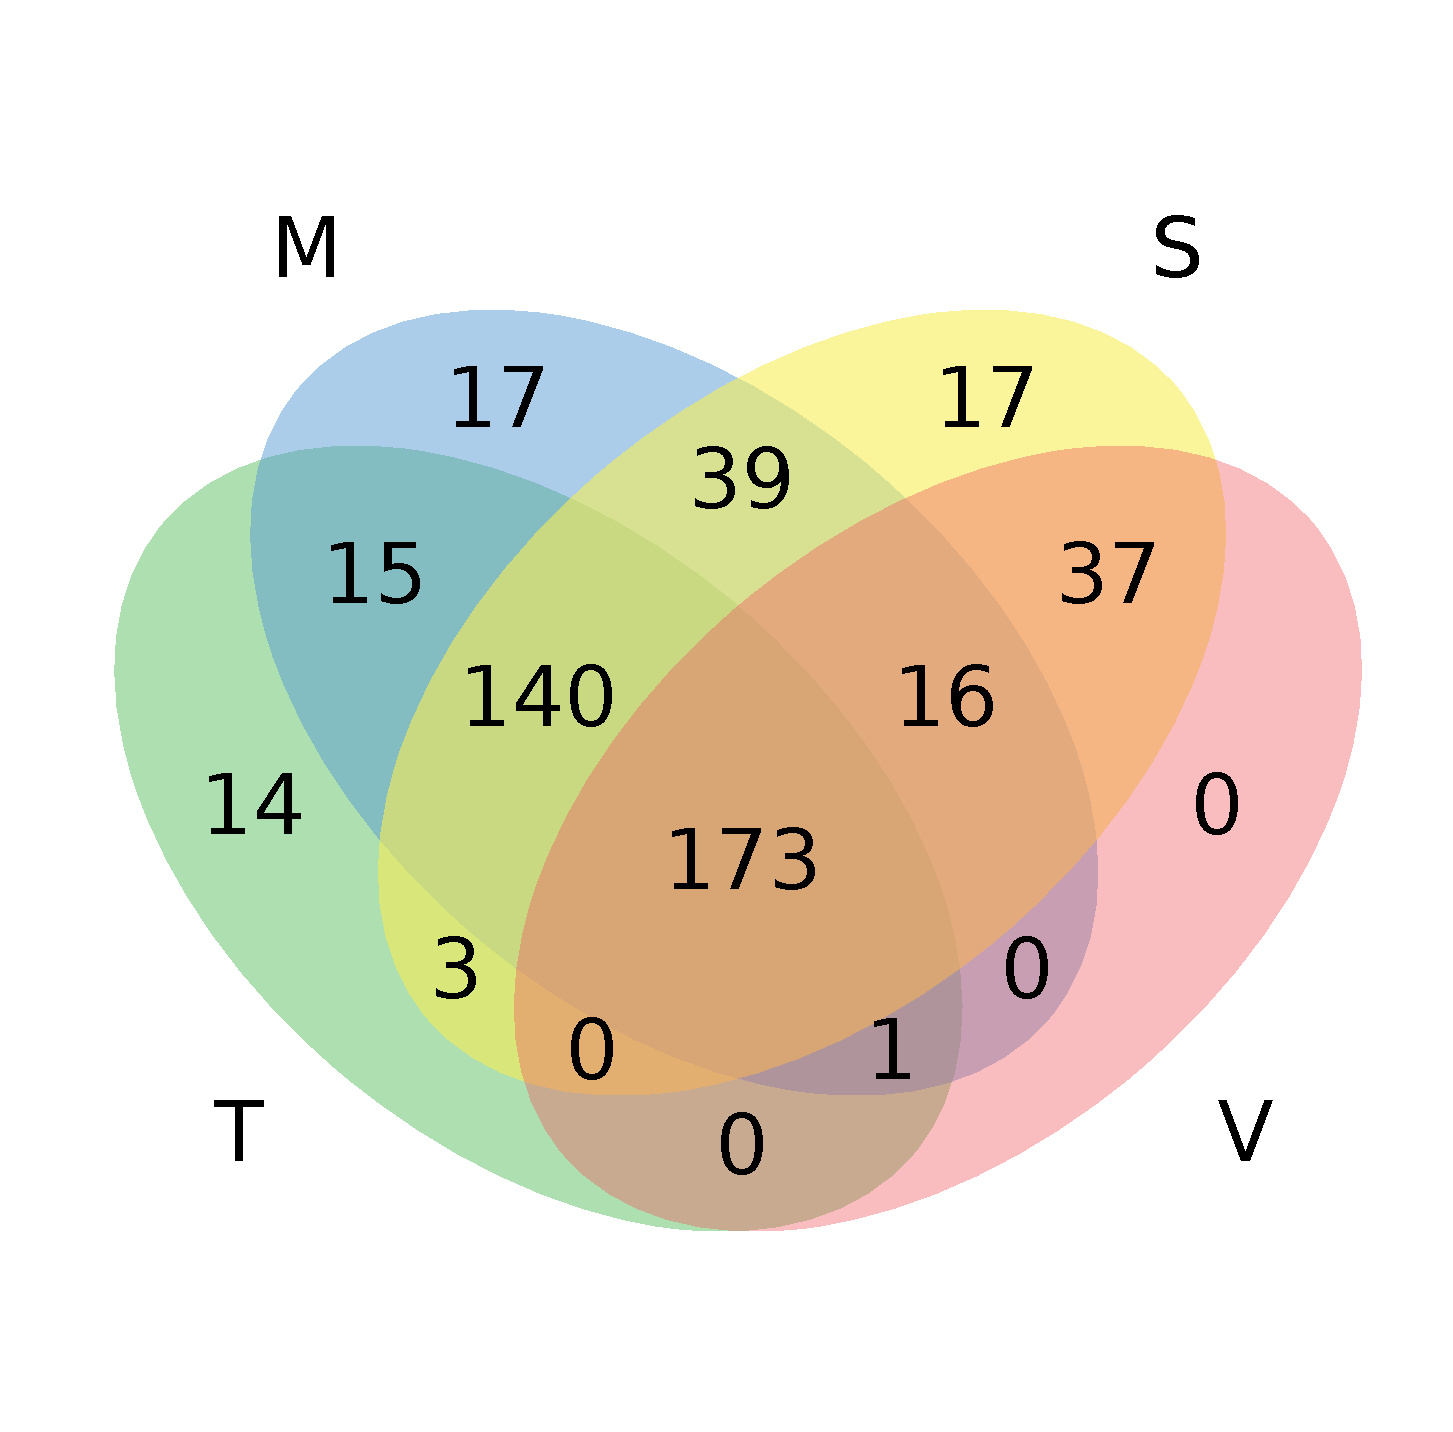
\includegraphics[width=\textwidth]{figures/venn_pma.pdf}
        \caption{\scriptsize{phpMyAdmin 4.7.0}}
        \label{fig:venn_pma}
    \end{subfigure}
    \begin{subfigure}[b]{0.22\textwidth}
          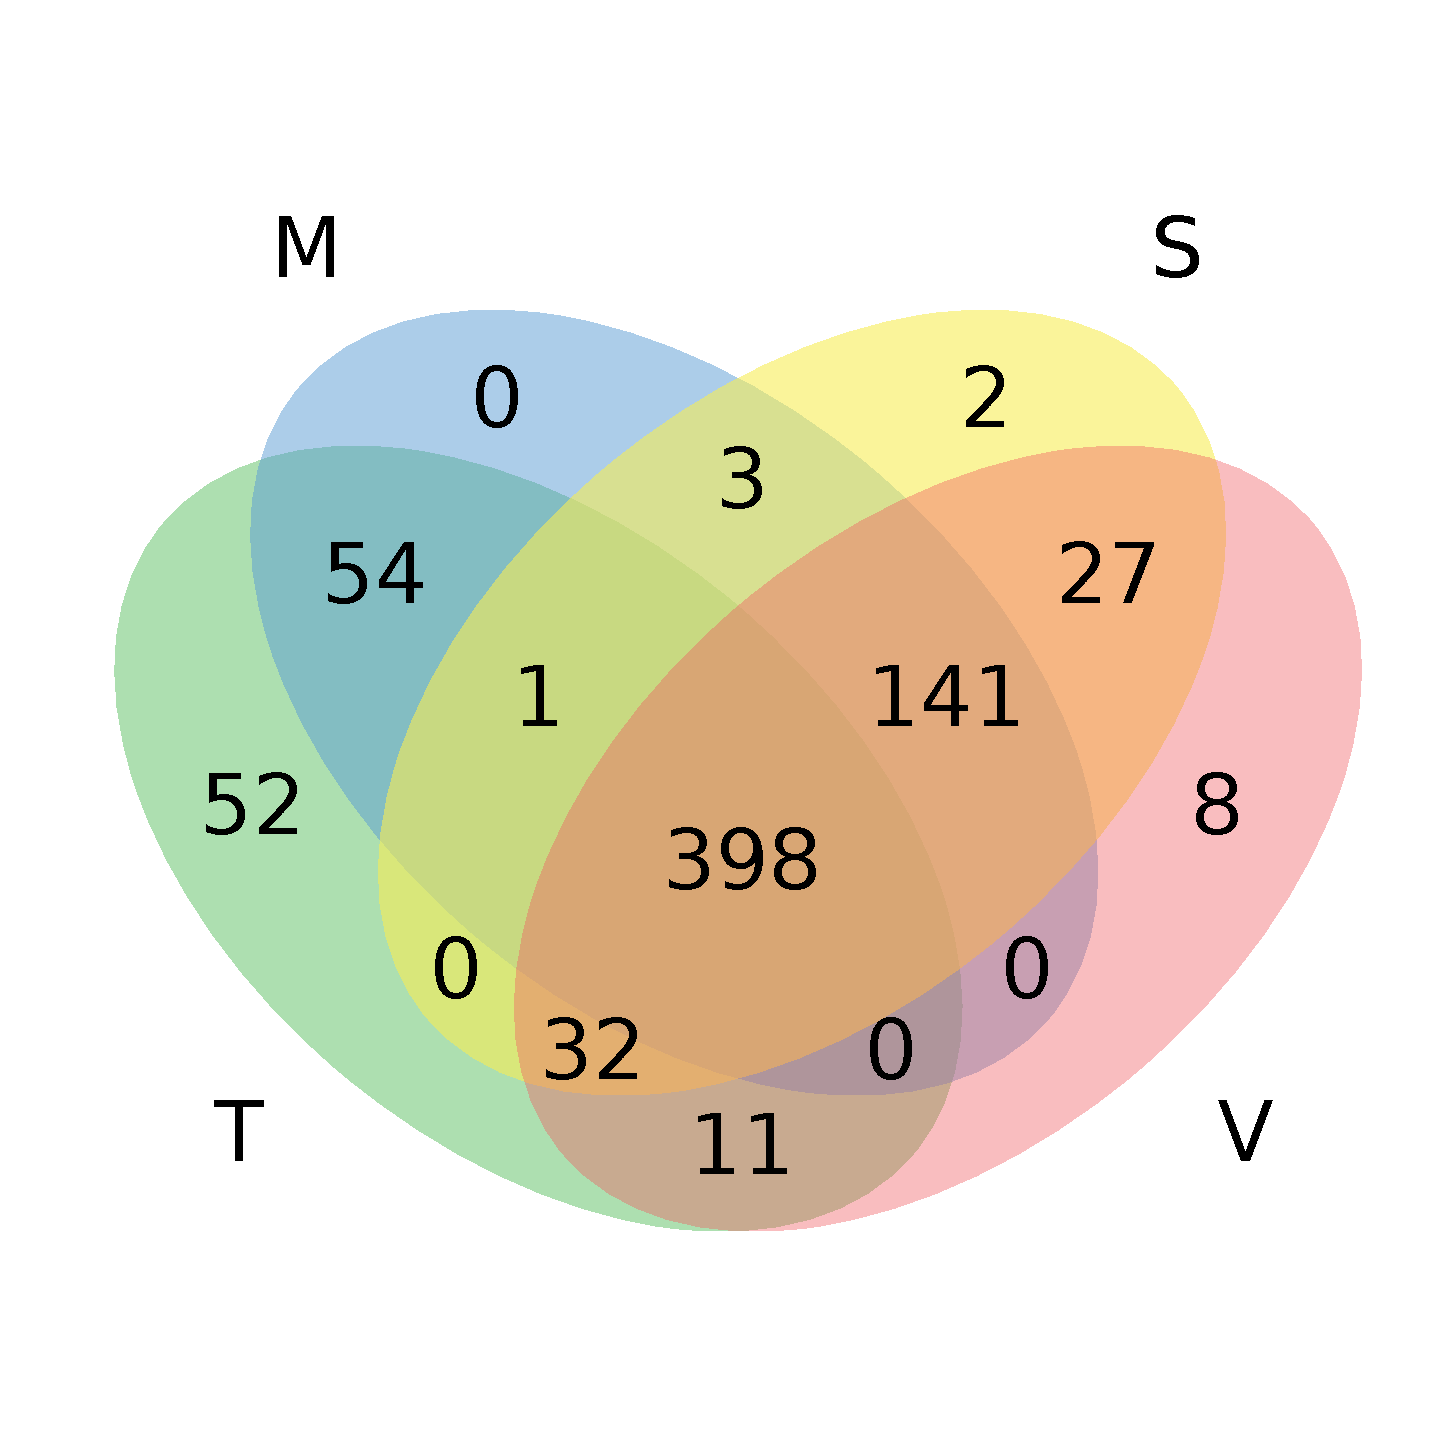
\includegraphics[width=\textwidth]{figures/venn_mwk.pdf}
          \caption{\scriptsize{MediaWiki 1.28.0}}
          \label{fig:venn_mwk}
    \end{subfigure}
    \begin{subfigure}[b]{0.22\textwidth}
          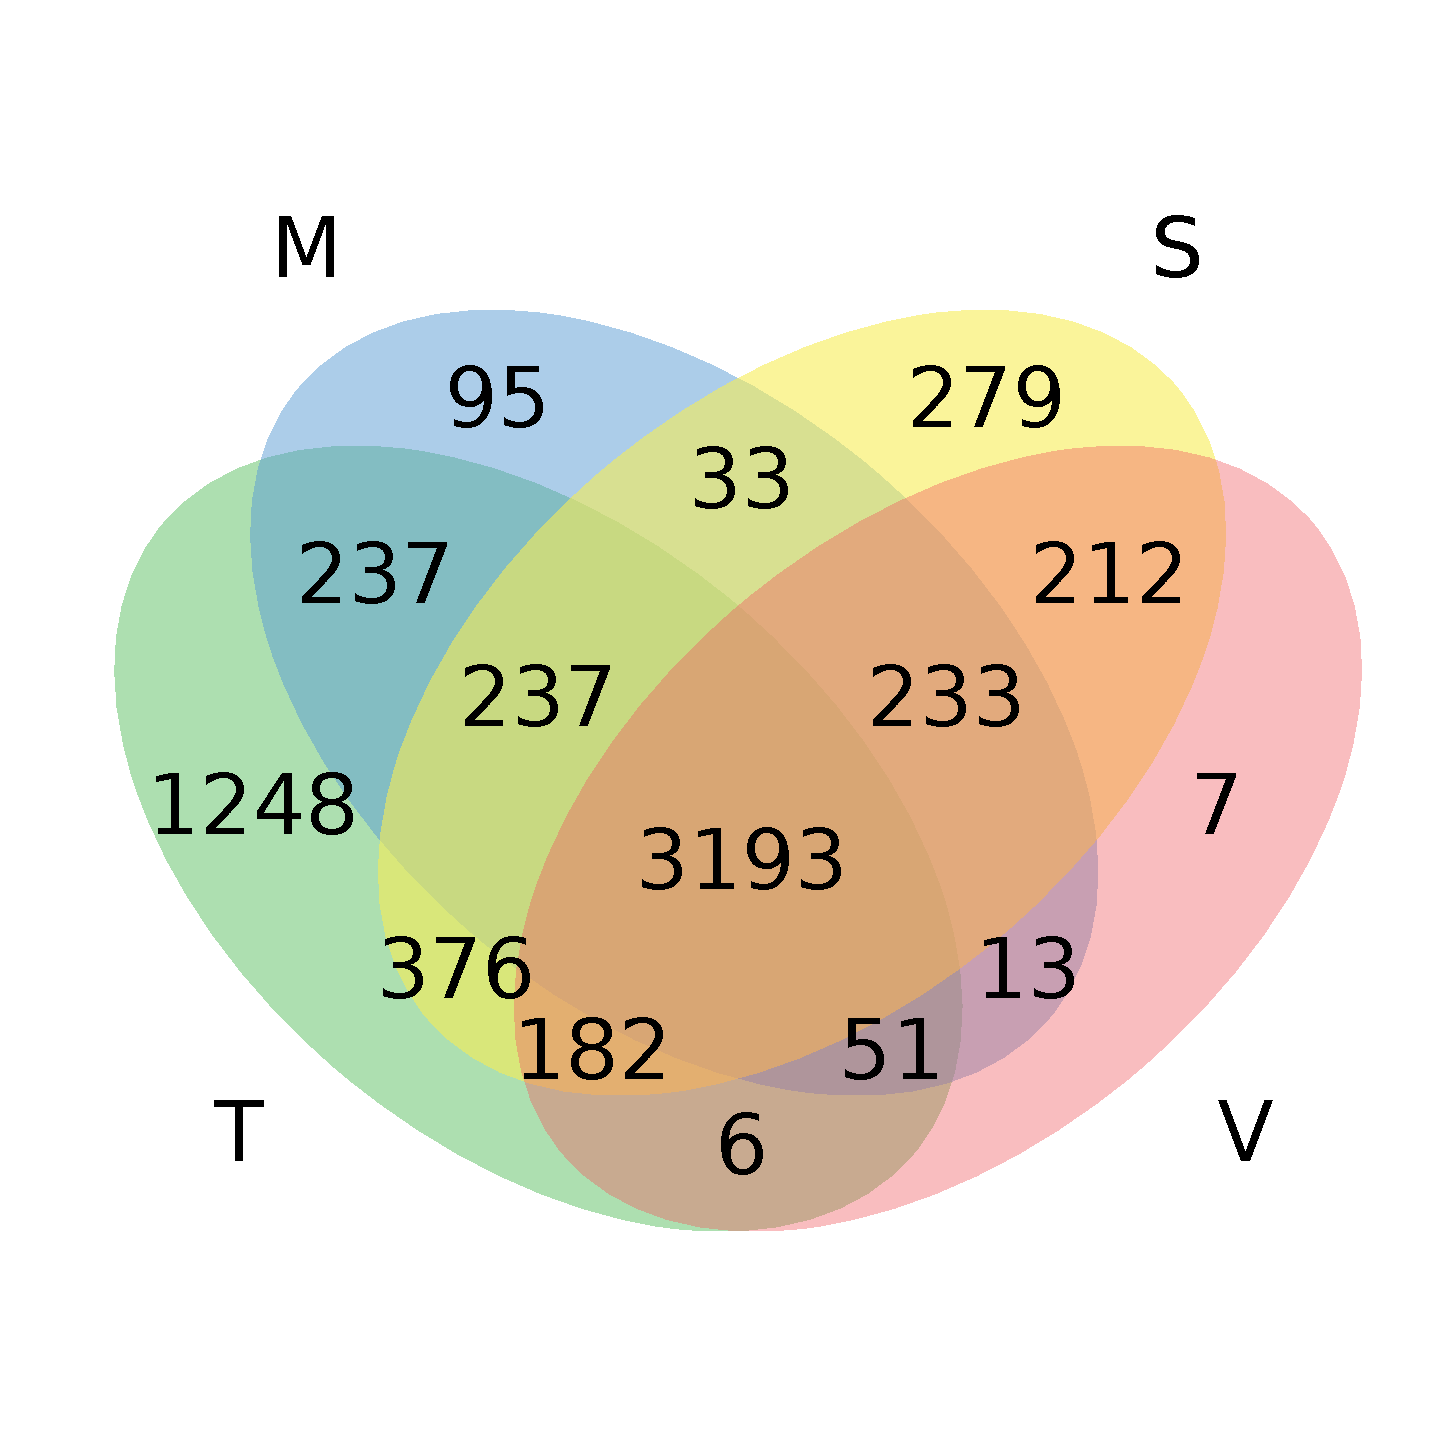
\includegraphics[width=\textwidth]{figures/venn_mgt.pdf}
          \caption{\scriptsize{Magento 2.0.5}}
          \label{fig:venn_mgt}
    \end{subfigure}
    \begin{subfigure}[b]{0.22\textwidth}
          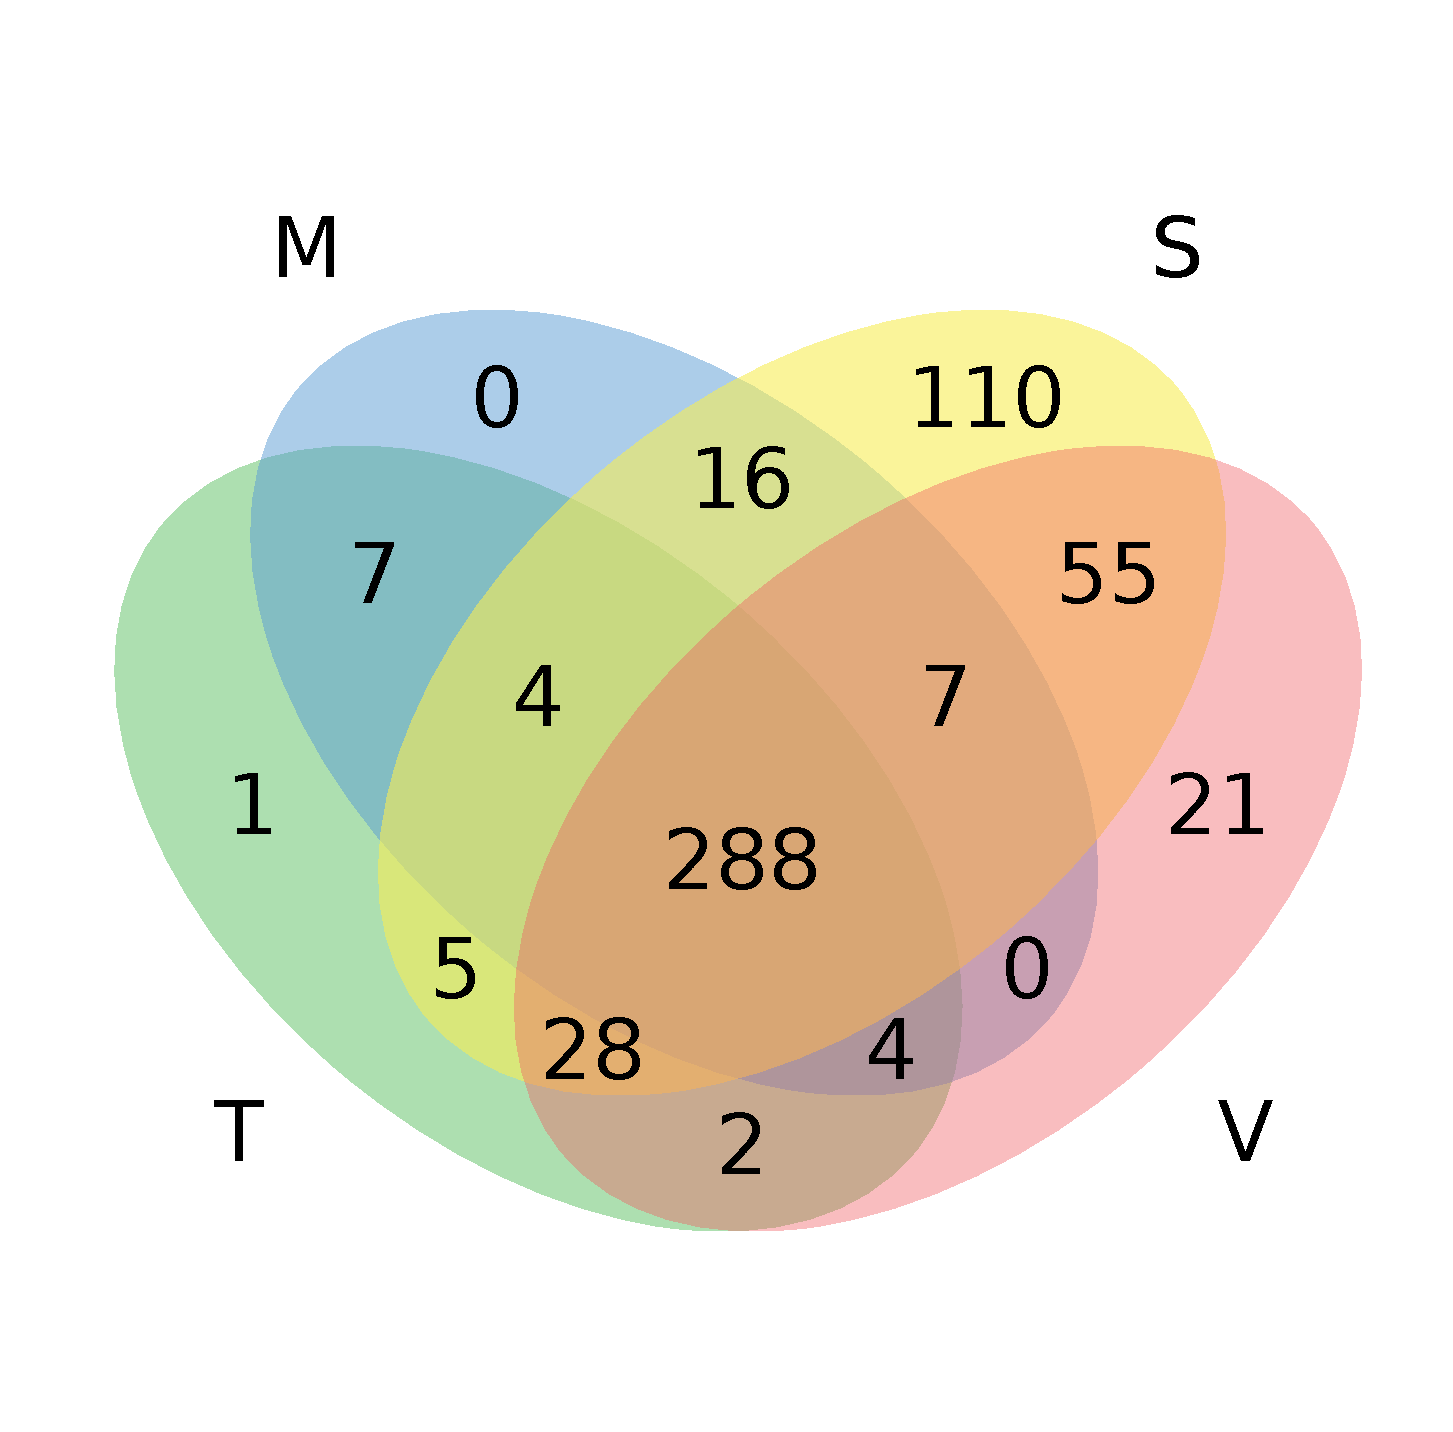
\includegraphics[width=\textwidth]{figures/venn_wp.pdf}
          \caption{\scriptsize{WordPress 4.7.1}}
          \label{fig:venn_wp}
    \end{subfigure}
  \caption{Venn Diagrams showing covered files during the execution of Tutorials, Crawler, Monkey testing and Vulnerability scanner}
  \label{fig:venncoverage}
\end{figure}

\subsection{Tutorials vs. Monkey Testing vs. Crawling vs. Vulnerability Scanning}
As described in Section~\ref{subsec:profiling}, to ensure that we exercise web applications in an objective and repeatable way, we utilized tutorials, monkey testing, crawlers, and vulnerability scanners. Figure~\ref{fig:venncoverage} shows the coverage, in terms of server-side files, that each method obtained on the latest version of each web application in our testbed. We can clearly see that all four methods are required, with each method contributing differently for different web applications.
For example, tutorials trigger more files in Magento compared to other applications, while Spider covers most unique files in WordPress.


\subsection{Debloating by the numbers}
To evaluate the effectiveness of our two debloating strategies, we computed different metrics that provide
insights into what has actually been removed during the debloating process.


\subsubsection{Logical lines of code}
\label{subsubsec:lloc}
The size of a program positively correlates with the number of programming errors (i.e. bugs). According to McConnel~\cite{mcconnell2004code}, the industry average, at least in 2004, was to have between 1 and 25 bugs for every one thousands lines of code. Given the importance of the size of an application to its overall security, we start by estimating the reduction of the attack surface by looking at the
Logical Lines Of Code (LLOC, sometimes also called Effective Lines Of
Code). LLOC is intended to measure lines of code without comments, empty
lines and syntactic structure required by the programming language. LLOC
reduction is a robust and precise indicator of how much the volume of
the code was reduced.
Figure~\ref{fig:lloc} reports on the LLOC for all versions of the applications
we debloated.

\paragraph{Number of logical lines over time.}
Looking at the number of LLOC of the original applications, we can observe two different evolution behaviors.
For WordPress, the amount of code is stable and there is even a small decrease of 2\% of LLOC between versions 4.7 and 4.7.1.
For the other applications, we observe the opposite where the source code in the latest versions spikes, compared to the ones released just before them: 82\% LLOC increase for phpMyAdmin, 99\% for MediaWiki, and 171\% for Magento. By
analyzing the code of these newer versions in an attempt to understand their
sudden expansion in size, we discovered that these spikes can be attributed to
a change in development practices, namely the reliance on external packages.
As WordPress does not rely on external packages, it does not exhibit this kind of behavior. We
discuss the issue of relying on external packages in more detail in Section~\ref{subsec:external}.


\begin{figure}[t]
  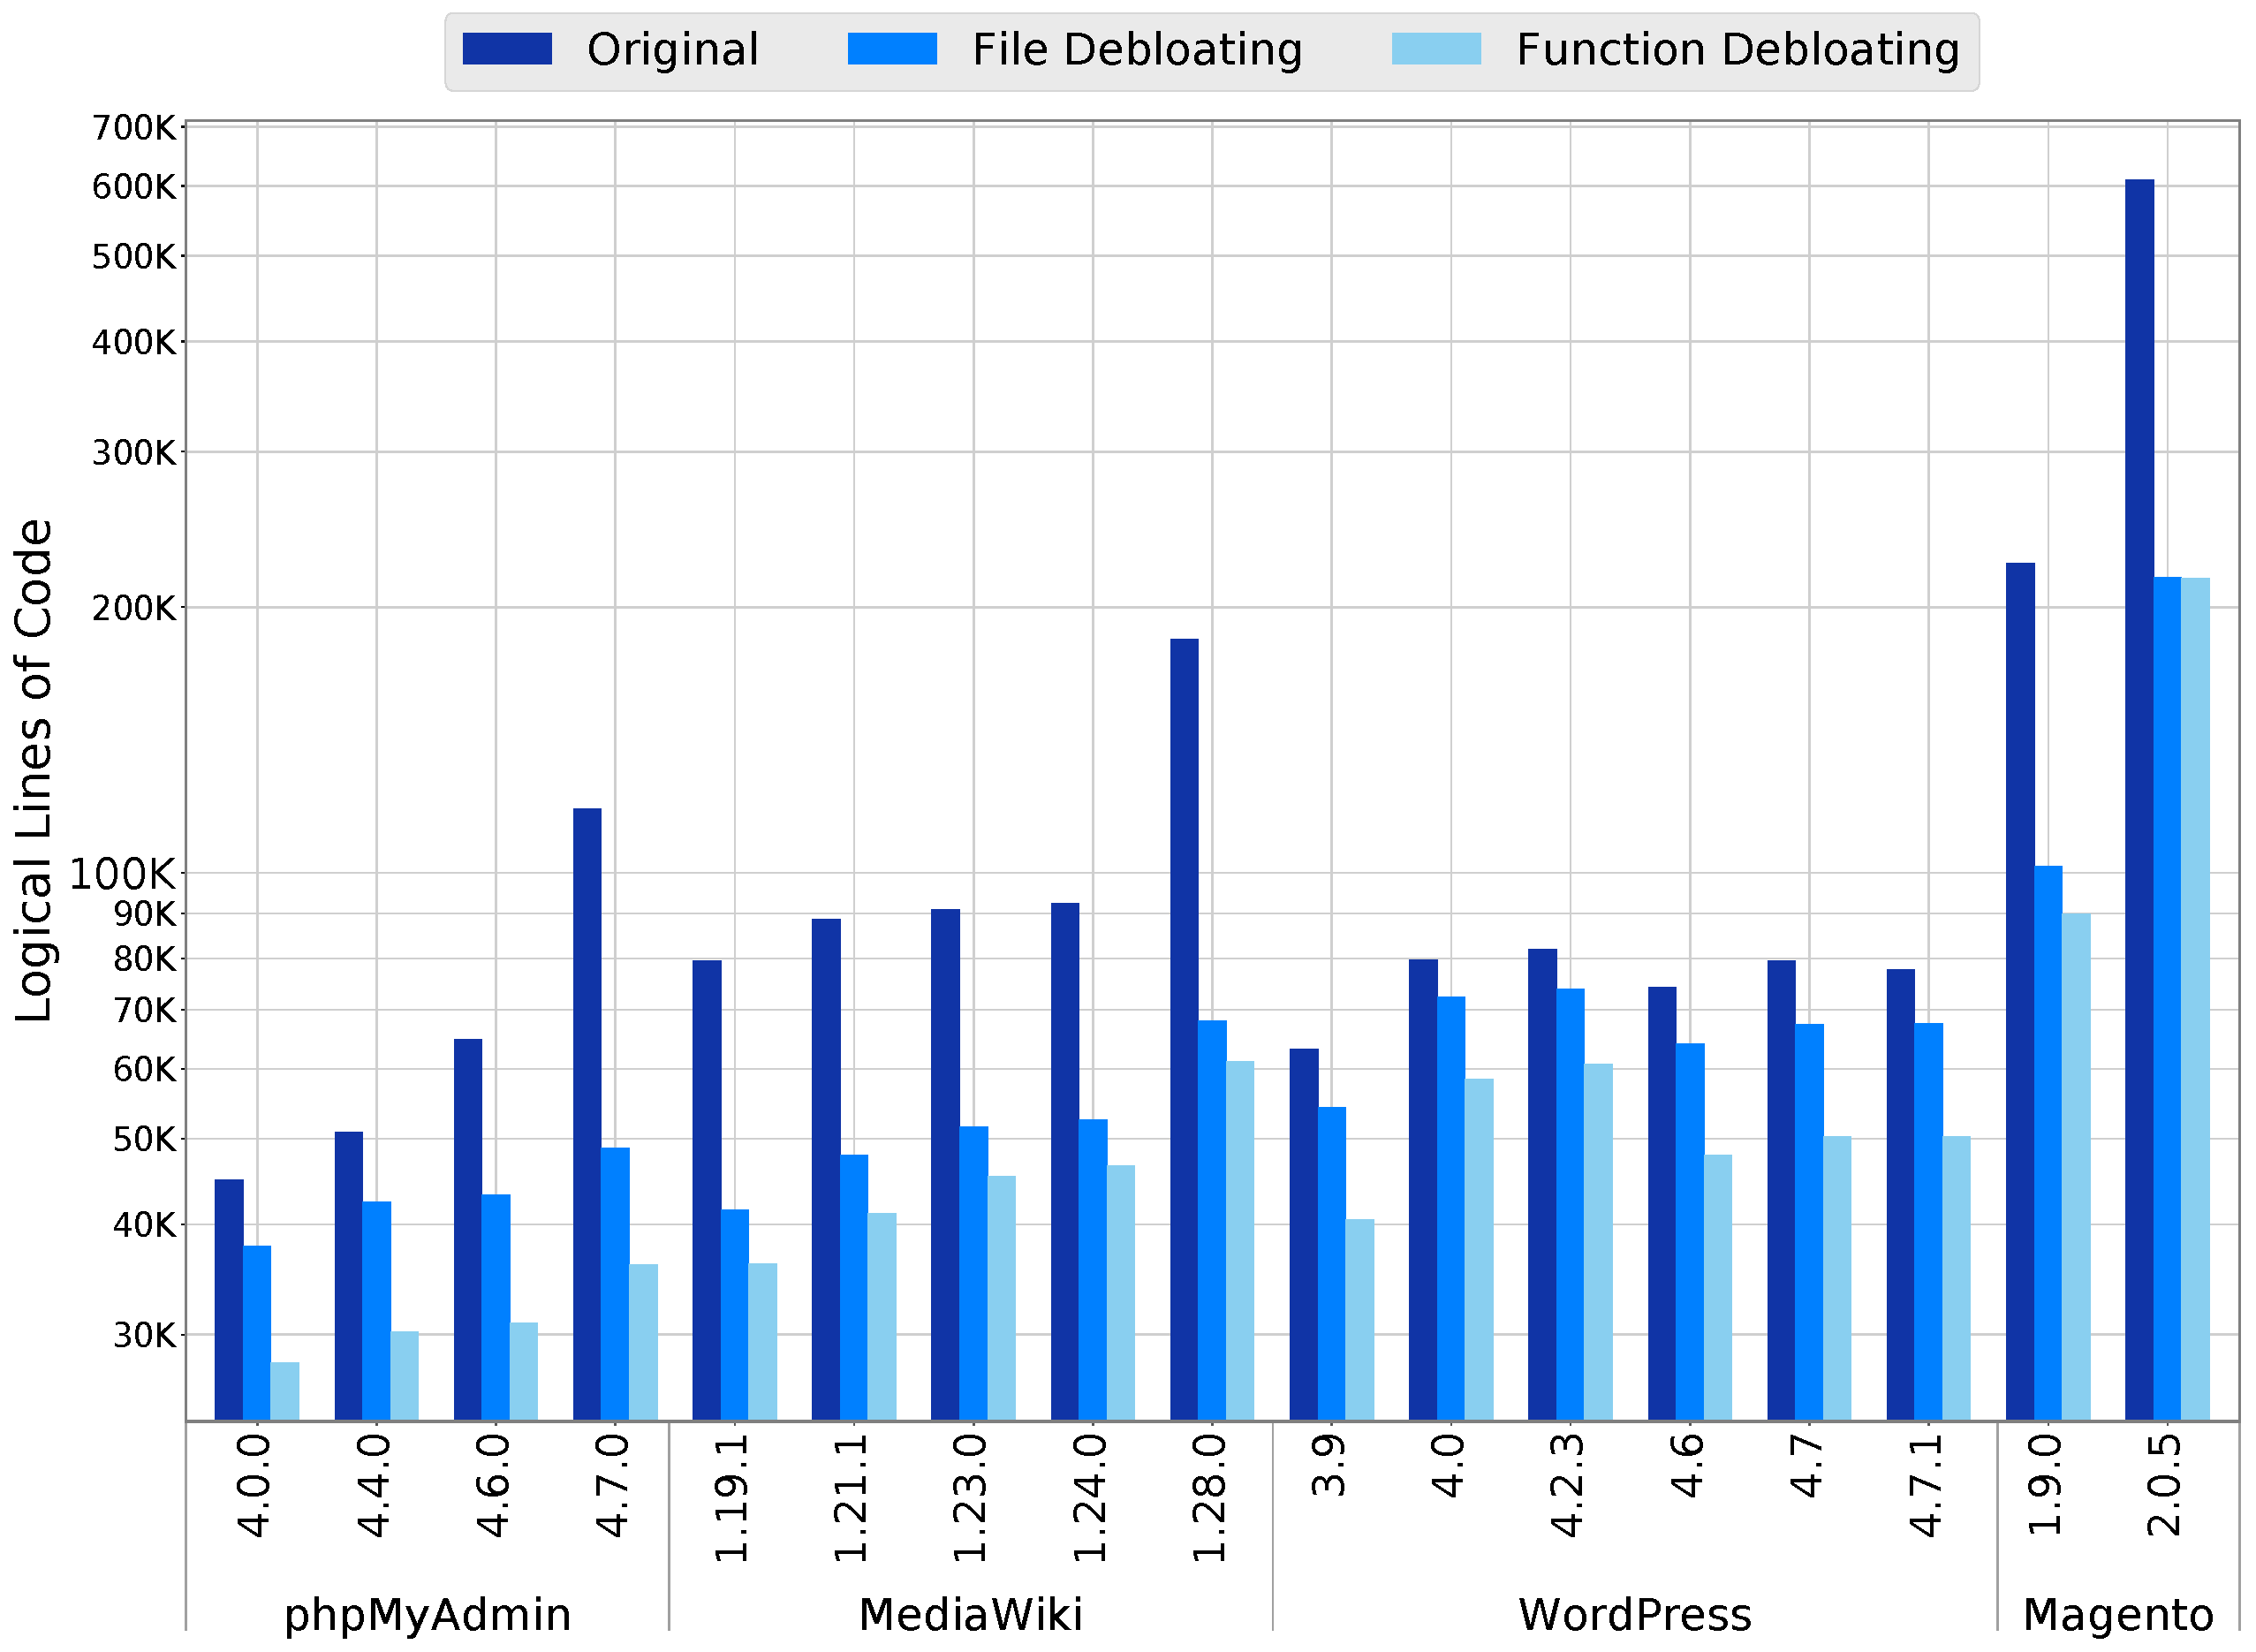
\includegraphics[width=\linewidth]{figures/lloc.pdf}
  \caption{Logical Lines of Code before and after debloating}
  \label{fig:lloc}
\end{figure}


\paragraph{File-level debloating.}
Overall, file-level debloating, the most conservative of the two evaluated
debloating strategies, is already effective in reducing the number of LLOC with an average of 33.1\% reduction.
The minimum observed in our experiment is 9.2\% for WordPress
v.4.0 and a maximum of 64.5\% for Magento v.2.0.5. For Magento,
this reduction represents a removal of 393K lines of code.
This number is a clear sign that large web applications encompass many
different features that may not be used by all users and therefore result
in bloated applications with an unnecessarily large attack surface. At the same time, it is worthwhile repeating that all debloating results presented in this section are conditional to how web applications are used. Therefore, these large levels of debloating cannot be guaranteed for all possible deployments of web applications. We discuss this issue in Section~\ref{sec:limitations}.

\paragraph{Function-level debloating.}
On average, function-level debloating is able to remove 46.8\% of lines of code.
For both Magento and MediaWiki, it can remove up to
7\% more code over file-level debloating. For phpMyAdmin and WordPress, we observe an
increase of debloating capability of up to 24\%. This
larger reduction (compared to MediaWiki and Magento) is mainly due to
the differences in software development practices.

Compared to the other
tested applications, phpMyAdmin and WordPress are more monolithic with a smaller number of large
source-code files. Since file-level debloating only removes files when none
of their functions were executed, the monolithic nature of these two applications resists
this kind of coarse-level debloating. Contrastingly, Magento and MediaWiki
are developed in a much more modular fashion (many small files each responsible
for a small number of well-defined tasks) and therefore lend themselves better to file-level
debloating. The more fine-grained, function-level debloating bypasses this
issue and can therefore reduce the attack surface of a web application,
even for more monolithic web applications.


\subsubsection{Cyclomatic complexity}
\label{subsubsec:cyclomatic-complexity}
Next, we look at the evolution of cyclomatic complexity (CC). CC is defined as
the number of linearly independent paths through the code of
an application~\cite{mccabe1976complexity}. A high CC for a
single class implies complicated code that is difficult to
debug and maintain~\cite{gill1991cyclomatic} and therefore
more prone to contain vulnerabilities when compared to code with low
CC~\cite{shin2008empirical,kurmus2013attack}.

\begin{figure}[t]
  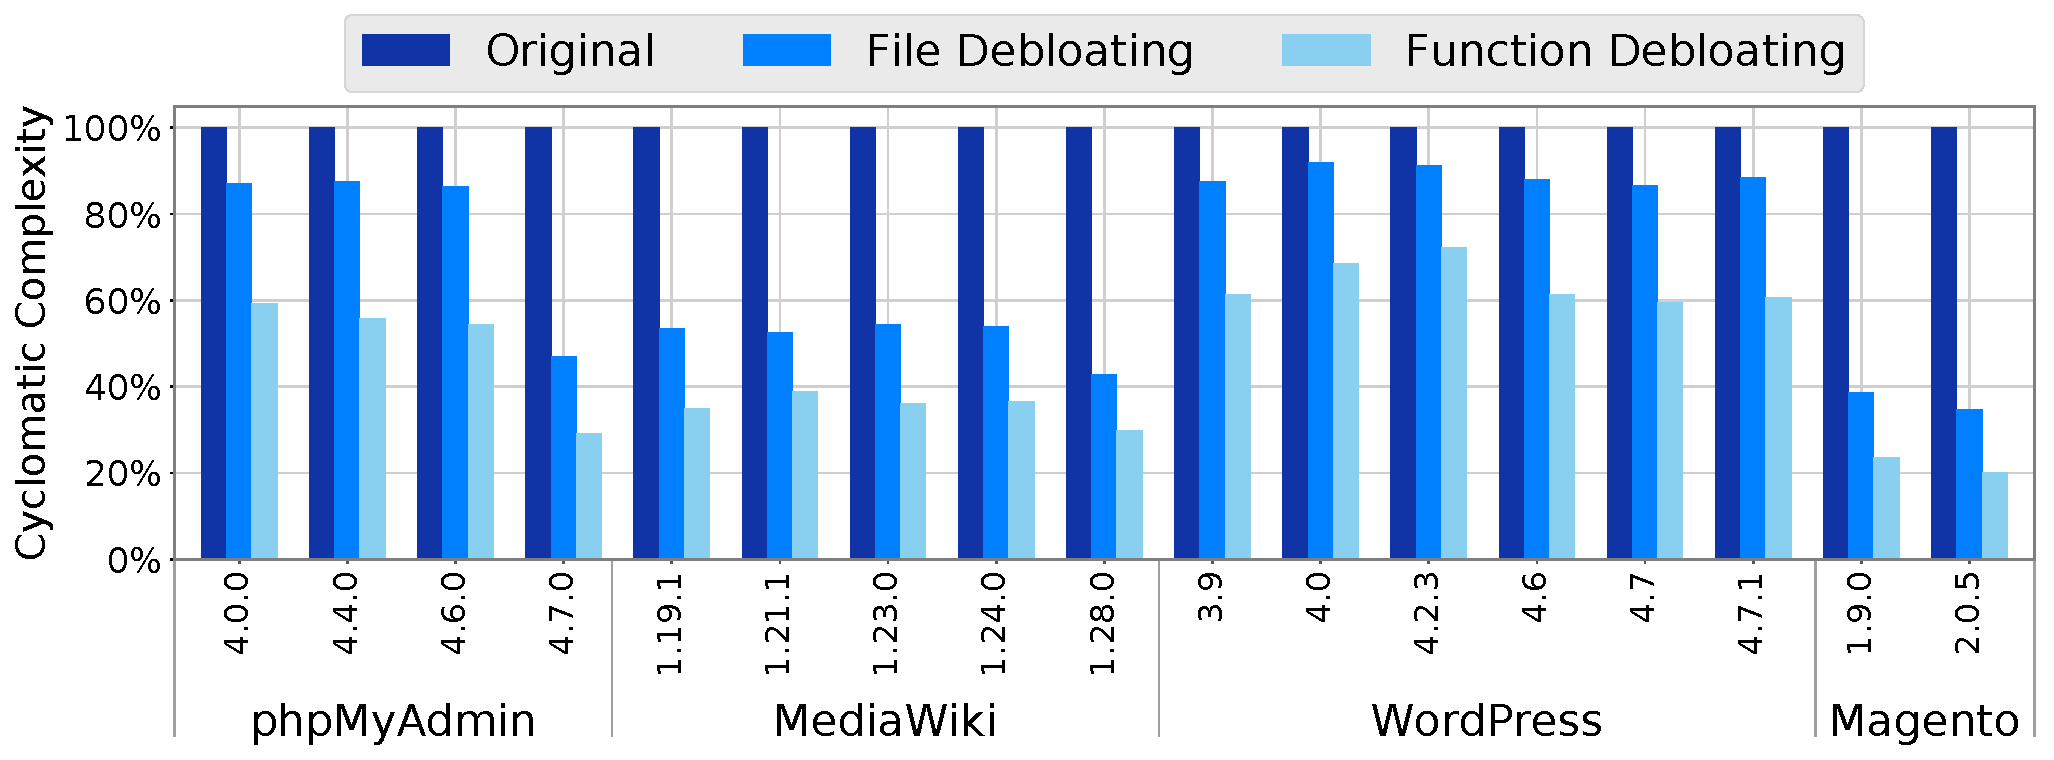
\includegraphics[width=\linewidth]{figures/cc_over_loc.pdf}
  \caption{Evolution of cyclomatic complexity before and after debloating}
  \label{fig:ccoverloc}
\end{figure}

Figure~\ref{fig:ccoverloc} reports on the evolution of the overall CC for
each tested version in our experiment. File-level debloating decreases
CC between 5.9\% to 74.3\% with an average of 32.5\%.
Function-level debloating decreases the program complexity between 23.8\% and 80.2\% with an average of 50.3\%.
These statistics demonstrate that
debloating can remove complex instructions and execution paths in addition to
simple ones. Moreover, the difference between file-level and function-level
debloating shows that code removal through function-level debloating is much
more suited to all kinds of web applications as shown earlier through LLOC
reduction achieved via function-level debloating.


\subsection{Analysis of CVEs}
In this section, we investigate the number of removed CVEs after debloating
along with the effects of debloating on different vulnerability categories.

\subsubsection{CVE reduction after debloating}
\label{sec:cve_reduction}
One practical way to measure the security benefits of debloating web
applications is to study the effects of debloating on known historical
vulnerabilities. If vulnerabilities were part of the core functionality of the
program, the evaluated debloating strategies will not be able to remove the
code associated with them. However, if some vulnerabilities reside in parts
of a web application that are not commonly used, the process of debloating
can effectively remove them.


Table~\ref{table:debloatingcvesresults} compares the effectiveness of
debloating strategies by listing the fractions of removed CVEs. We consider
a vulnerability to have been successfully removed if all the lines of code
and functions associated with that vulnerability were removed during the
stage of debloating. This is a conservative approach as one modification
performed on a single line could thwart a complete attack. As such, the
numbers we report in this section can be interpreted as lower bounds of
the actual number of removed CVEs.

\begin{table}[t]
\caption{Number of CVEs removed after application debloating}
\centering
\begin{tabular}{|c|l|l|l|l|l|}
\hline
\multicolumn{1}{|l|}{\textbf{Application}} & \textbf{Strategy}   & \multicolumn{2}{l|}{\begin{tabular}[c]{@{}l@{}}\textbf{Total}\\ \textbf{Removed CVEs}\end{tabular}} & \multicolumn{2}{l|}{\begin{tabular}[c]{@{}l@{}}\textbf{Removed}\\ \textbf{Exploitable CVEs}\end{tabular}} \\ \hline
\multirow{2}{*}{phpMyAdmin}       & File Debloating     & 4/20                                    & 20 \%                                   & 3/19                                      & 15.7 \%                                     \\ \cline{2-6}
                                  & Function Debloating & 12/20                                   & 60 \%                                   & 11/19                                     & 57.8 \%                                     \\ \hline
\multirow{2}{*}{MediaWiki}        & File Debloating     & 8/21                                    & 38 \%                                   & 3/16                                      & 18.7 \%                                     \\ \cline{2-6}
                                  & Function Debloating & 10/21                                   & 47.6 \%                                 & 5/16                                      & 31.2 \%                                     \\ \hline
\multirow{2}{*}{WordPress}        & File Debloating     & 0/20                                    & 0 \%                                    & 0/20                                      & 0 \%                                        \\ \cline{2-6}
                                  & Function Debloating & 2/20                                    & 10 \%                                   & 2/20                                      & 10 \%                                       \\ \hline
\multirow{2}{*}{Magento}          & File Debloating     & 1/8                                     & 12.5 \%                                 & 1/8                                       & 12.5 \%                                     \\ \cline{2-6}
                                  & Function Debloating & 3/8                                     & 37.5 \%                                 & 3/8                                       & 37.5 \%                                     \\ \hline
\end{tabular}
\label{table:debloatingcvesresults}
\end{table}

In terms of configuration, we selected the default one for each application.
However, certain vulnerabilities may not be exploitable under this configuration.
For example, there exists 5 CVEs in our dataset for MediaWiki which require file upload functionality to be enabled. Since this option is disabled by default, we make an explicit distinction in the table.
``Total Removed CVEs'' is the total number of CVEs removed by debloating regardless of whether the vulnerable code is enabled or disabled through a configuration option. ``Removed Exploitable CVEs'' reports on the CVEs that are reachable under default configurations of target web applications.

On average, we discovered that up to 38~\% of vulnerabilities are removed by
file debloating whereas 10-60~\% are removed by function debloating. As
shown in Table~\ref{table:debloatingcvesresults}, function-level debloating
can triple (in the case of phpMyAdmin and Magento) the number of removed CVEs, compared to file-level debloating. This
behavior can be generalized to web applications that do not have CVE
information and demonstrates that the reduction of a web application's
LLOC (Section~\ref{subsubsec:lloc}) and its cyclomatic complexity
(Section~\ref{subsubsec:cyclomatic-complexity}) translates to a reduction
of concrete vulnerabilities. Wordpress is a clear negative outlier with only
10\% CVE reduction, even through the more flexible function-debloating
strategy. As mentioned earlier, WordPress is a relatively monolithic
application and most of our mapped CVEs are located in core WordPress code (e.g.,
Authentication, CSRF tokens, and post/comment-related actions) which cannot
be removed by our debloating framework.

\begin{figure}[t]
  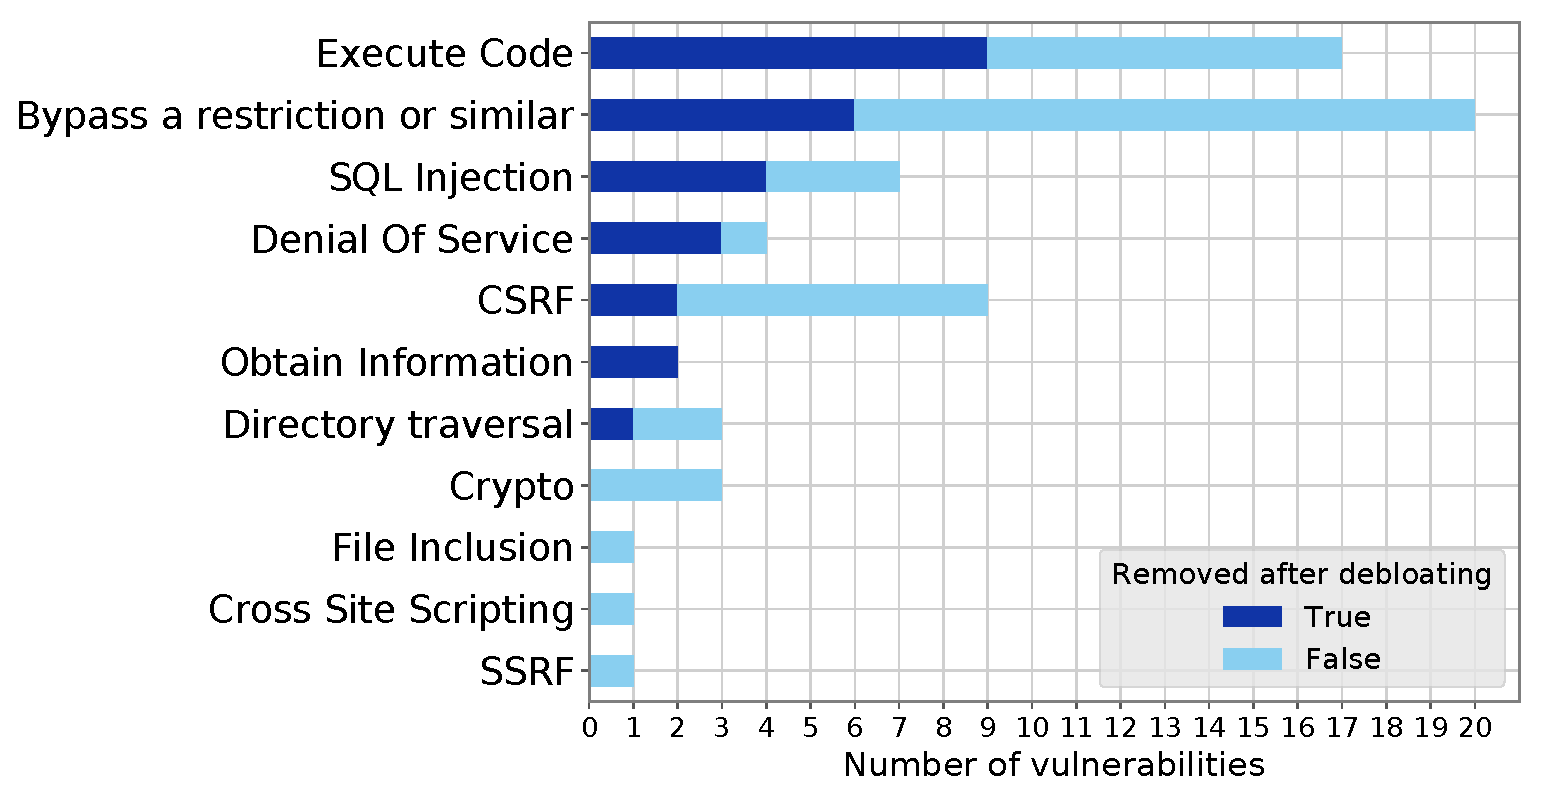
\includegraphics[width=\linewidth]{figures/vuln_per_category.pdf}
  \caption{Vulnerability Categories}
  \label{fig:vulnpercat}
\end{figure}

\subsubsection{Types of CVEs in analyzed web applications}

Even though our results demonstrate the ability to remove vulnerabilities
from web applications through the use of debloating, one may wonder
whether debloating is better suited for some types of vulnerabilities over
others. Figure~\ref{fig:vulnpercat} provides details on the categories of
the CVEs we removed through debloating.


One can observe that for certain classes of vulnerabilities, such as,
Denial-of-Service attacks and Information-Revealing vulnerabilities,
debloating can almost completely remove them.
For others, such as, restriction bypassing, command execution, and
SQL injection, debloating can substantially reduce them.
Our interpretation of these findings has to do with the maturity of
the evaluated web applications. Specifically, all four web applications
have been available for a long period of time, allowing many shallow
vulnerabilities to have already been discovered and corrected. The remaining
vulnerabilities are likely to be situated in parts of a web application that
are less commonly exercised. For example, the code-execution vulnerabilities
that can be removed for phpMyAdmin are inside very specific features, such as,
the ability to export PHP arrays (CVE-2016-6609), the support of the
ZIP extension while importing data (CVE-2016-6633), and the abilities
to copy table definitions (CVE-2013-3238) and perform Regex search and replace over table columns
(CVE-2016-5734).

\begin{table*}[t]
\caption{Statistics on the external packages included in web applications and the effects of debloating in terms of reducing their LLOC.}
\centering
\scalebox{0.57}{
\begin{tabular}{c|c|c|c|c|c|c|c|c|c|}
\cline{2-10}
 & \multicolumn{3}{c|}{\textbf{Before debloating}} & \multicolumn{6}{c|}{\textbf{After function-level debloating}} \\ \hline
\multicolumn{1}{|c|}{\multirow{2}{*}{\textbf{Application}}} & \multirow{2}{*}{\begin{tabular}[c]{@{}c@{}}\# \textit{lines in main}\\\textit{application}\end{tabular}} & \multirow{2}{*}{\begin{tabular}[c]{@{}c@{}}\textit{\# lines in}\\\textit{packages}\end{tabular}} & \multirow{2}{*}{\textit{\# packages}} & \multirow{2}{*}{\begin{tabular}[c]{@{}c@{}}\textit{\# lines in main}\\ \textit{application}\end{tabular}} & \multirow{2}{*}{\begin{tabular}[c]{@{}c@{}}\textit{\# lines in}\\\textit{packages}\end{tabular}} & \multirow{2}{*}{\begin{tabular}[c]{@{}c@{}}\textit{\# packages}\\\textit{completely}\\\textit{removed}\end{tabular}} & \multicolumn{3}{c|}{\begin{tabular}[c]{@{}c@{}}\textit{\# packages where a given \%}\\\textit{lines were removed}\end{tabular}} \\ \cline{8-10}
\multicolumn{1}{|c|}{} &  &  &  &  &  &  & \textgreater{}\textit{70\%} & \begin{tabular}[c]{@{}c@{}}\textless{}\textit{70\% and}\\ \textgreater{}\textit{30\%}\end{tabular} & \textless{}\textit{30\%}\\ \hline
\multicolumn{1}{|c|}{phpMyAdmin 4.7.0} & 35,739  & 82,604  & 45 & 26,377 (-26.2\%)  & 9,653 (-88.3\%)  & 38 (84.4\%) & 2 & 1  & 4  \\ \hline
\multicolumn{1}{|c|}{MediaWiki 1.28.0} & 133,019 & 50,898  & 40 & 54,827 (-58.8\%)  & 6,285 (-87.7\%)  & 24 (60.0\%) & 2 & 2  & 12 \\ \hline
\multicolumn{1}{|c|}{Magento 2.0.5}    & 396,448 & 212,906 & 71 & 181,696 (-54.2\%) & 34,038 (-84.0\%) & 58 (81.7\%) & 6 & 5  & 2  \\ \hline
\end{tabular}
}
\label{table:numberofpackages}
\end{table*}


Contrastingly, the three cryptography-related vulnerabilities we analyzed are
still present in the debloated versions of web applications. One of the CVEs
related to this category is about a flaw in the cookie encryption algorithm in
phpMyAdmin (CVE-2016-6606). Since every page interacts with user
cookies to, at the very least, verify them, vulnerable code cannot be
removed. Another vulnerability in this category relates to an insecure random
number generator used in cryptographic operations by Magento (CVE-2016-6485).
This vulnerability exists in a constructor of the main encryption
classes which is widely used throughout the application. When considered
together, these findings suggest that cryptography-related vulnerabilities
are a core part of web applications and thus unlikely to be removed through
the process of debloating.

\subsection{External packages}
\label{subsec:external}

\subsubsection{Quantifying the bloat from external packages}
In our testbed, phpMyAdmin v.4.7.0, MediaWiki v.1.28.0 and Magento v.2.0.5 rely
on external dependencies that can be downloaded via Composer (WordPress does not rely on external packages). As described in
Section~\ref{sec:background}, Composer is a package manager for PHP (similar
to the NPM manager for NodeJS applications) which allows web applications
to specify which external packages they rely on and have these packages be
tracked and updated.

As we briefly discussed in Section~\ref{subsubsec:lloc}, the number of LLOC of
these three specific versions dramatically
increases (compared to prior versions) because of this dependency on external
packages. Table~\ref{table:numberofpackages} provides statistics on the
number of packages pulled by these applications and how much bloat they
provide against our usage profiles.


First, one can observe that external packages introduce a large amount of
unused code. For all three debloated applications, more than 84\% of their code
was removed from them. This means that the attack surface is unnecessarily
large through the dependency on external packages. The number of removed
lines from external packages for Magento is particularly noteworthy with
more than 178,000 lines of code removed. Moreover, the number of packages
that can be completely removed is also quite large: 84\% for phpMyAdmin,
60\% for MediaWiki and 81\% for Magento. This confirms that most packages
are unnecessary for the usage profiles that we recorded. Finally, focusing
exclusively on the lines of code, phpMyAdmin is the only application where
external packages have more lines than the main application. However, after
debloating, this relationship is reversed with the codebase of phpMyAdmin
being three times the size of the introduced external packages.


Despite the advantages of using package managers (e.g. the ability to track
dependencies and update vulnerable libraries without the need to update
the main application), our findings show that these advantages come at a
considerable cost in terms of unnecessarily expanding the attack surface of
a web application with code that is seldomly executed. As such, developers
must take special care to include the bare minimum of external packages,
knowing the unwanted side-effects that each external package brings.

\subsubsection{Removing POI gadgets}

\paragraph{What are POI gadgets?}
Property Oriented Programing (POP) is an exploitation technique
in PHP which works similarly to Return Oriented Programming
(ROP)~\cite{shacham2007geometry} and is used to exploit PHP Object Injection
(POI) vulnerabilities~\cite{POI}. In this technique, the attacker creates
exploit gadgets from available code in the applications. By chaining
multiple gadgets within the application, an attacker can usually run
arbitrary code, write to arbitrary files, or interact with a database. Dahse
et al. have studied the automatic generation of such gadget chains for PHP
applications~\cite{Dahse:2014:CRA:2660267.2660363}.

\paragraph{PHP unsafe deserialization.}
The PHP language gives developers the ability to serialize arbitrary objects in
order to store them as text, or transfer them over the network. Deserialization
reverses this process, generating PHP objects from serialized data. This
mechanism can be abused by an attacker to load specific classes in the
application and build a gadget chain. Practical examples of this vulnerability
are when \texttt{unserialize} is called on a database field or value of a
field within a cookie that can be manipulated by the users.

Historically, this attack was very difficult to successfully execute. Attackers
could only build gadgets with the classes that were present in the context of
the vulnerable file. They needed insights into how the application was built
in order to know which classes could be abused for gadgets. However, starting
from PHP 5, the \texttt{\_\_autoload()} magic function~\cite{PHPAutoload}
was introduced and unintentionally made exploitation of deserialization
vulnerabilities easier. This new loading feature was beneficial for PHP
developers who did not have to manually include all the files they wanted to
use at the very top of each of their PHP files. It also helped the adoption
of package managers like Composer, as any external dependency could be easily
called from anywhere in the application. The downside of this new function
was that it also allowed attackers to instantiate any PHP class across the
entire application thereby enabling the easier construction of gadget chains.

In order to build a chain, attackers use these so-called ``magic''
functions~\cite{PHPWakeup} that form the basis of their gadget chain. One of
the functions that is widely used in POI exploits is the \textit{destruct}
function. In Section~\ref{subsec:coverage}, we detailed the challenges in
getting complete coverage of destructors in our tested applications. Accurate
coverage of destructors also allows us to precisely analyze the impact of
debloating on gadget creation.

\paragraph{Can debloating remove gadgets from external packages?}

Given the increased footprint of web applications due to their reliance
on package managers and external dependencies, one may wonder about the
possibility of abuse of these packages for the creation of gadgets. To
measure the effect of debloating on Property-Oriented-Programming (POP)
gadgets, we utilized the PHPGGC~\cite{PHPGGC} library. PHPGGC (which stands
for PHP Generic Gadget Chains) contains a list of known gadgets in popular
PHP packages such as Doctrine, Symfony, Laravel, Yii and ZendFramework. When
a vulnerable PHP application includes any of the packages listed in PHPGGC,
the attackers can generate gadget chains to achieve RCE, arbitrary file
writes, and SQL injections.

We analyzed the available gadget chains in PHPGGC and
checked whether any of our tested PHP applications included these
chains. Table~\ref{table:knowngadgets} summarizes the presence of each gadget
and whether debloating removes them or not. WordPress is not included in this table because it does not rely on external packages.
This does not make WordPress immune to POI attacks, but universally known gadget chains in popular external packages can not be used to exploit WordPress.
For the affected applications, file-level debloating removes 4/6 gadgets while function debloating removes
6/6 available gadget chains. This again demonstrates the power of debloating
which can not only remove some fraction of vulnerabilities but also make
the exploitation of the remaining ones harder by removing the gadgets that
attackers could abuse during a POI attack.


\begin{table}[]
  \centering
  \caption{List of packages with known POP gadget chains}
\begin{tabular}{|l|l|c|c|}
\hline
\multirow{2}{*}{\textbf{Application}}      & \multirow{2}{*}{\textbf{Package}} & \multicolumn{2}{l|}{\begin{tabular}[c]{c@{}c@{}}\textbf{Removed by}\\\textbf{Debloating}\end{tabular}} \\ \cline{3-4}
    &    & \textit{File}     &  \textit{Function}                                     \\ \hline
\multirow{2}{*}{phpMyAdmin 4.7.0} & Doctrine                 & \faCheck                                         & \faCheck                                            \\ \cline{2-4}
                                  & Guzzle                   & \faCheck                                         & \faCheck                                            \\ \hline
MediaWiki 1.28.0                  & Monolog                  & \faCheck                                         & \faCheck                                            \\ \hline
\multirow{3}{*}{Magento 2.0.5}    & Doctrine                 & \faCheck                                         & \faCheck                                            \\ \cline{2-4}
                                  & Monolog                  & \faTimes                                         & \faCheck                                            \\ \cline{2-4}
                                  & Zendframework            & \faTimes                                         & \faCheck                                            \\ \hline
\end{tabular}
\label{table:knowngadgets}
\end{table}


\subsubsection{Utilizing development packages in production}
During our analysis of external packages, we identified yet another source
of bloat in new versions of web applications. When declaring external
dependencies through Composer, two options are available: ``require'' and
``require-dev''. The first option indicates packages that are mandatory for
the application to run properly. The second lists packages that should only be
used in development environments, such as, packages providing support for unit
testing, performance analysis, and profiling. We discovered that applications
downloaded from official websites often include these development packages. As
such, when these packages are used to deploy web applications in production
mode, they will contain unnecessary development libraries. This does not
only increase the attack surface by having unnecessary code bloating the
application, but can also lead to exploitation for misconfigured applications.

CVE-2017-9841 presents one example of such a
vulnerability~\cite{phpunitVulnerability}. Specifically, this CVE refers
to an RCE attack in specific versions of the PHPUnit library, which is
a popular unit testing library for PHP. By default, Composer places all
external packages under ``vendor'' directory. If this specific directory
happens to be accessible through a misconfiguration of the server, PHPUnit
files are then accessible and can be exploited to conduct an RCE attack.

The four web applications that we evaluated for this study, present
different behaviors with respect to development packages. WordPress does not rely on external packages downloaded through Composer.
MediaWiki never
included development packages in its releases. phpMyAdmin had them in version
4.7.0 but stopped including them in version 4.8.3 (the latest at the time of
writing). Magento started including them from version 2.0 and still includes
them today. We have reached out to Magento and informed them about this issue.


\subsection{Qualitative analysis of the removed code}
\label{subsec:qualitative}

In the previous sections, we analyzed the effects of debloating on the source code of applications from a software-engineering perspective (i.e. LLOC and Cyclomatic Complexity reduction) as well as from a security standpoint (i.e. number of CVEs and gadgets removed). At the same time, one may wonder what exactly was removed from each application during the process of debloating.



Given that thousands of files were removed, manually analyzing each file does not scale. As such, we turn to NLP techniques that allow us to cluster the removed files together and provide us with hints about the nature of each cluster. Specifically, we use the k-means clustering algorithm based on text vectors extracted from removed file names and file paths. Each file path includes directories that indicate which library or package, the file belongs to. For most modern web applications, this allows for a reasonable separation of files across different application plugins and modules.
To end up with meaningful clusters, we tuned TFIDF vectorizer parameters along with the number of k-means clusters. We used the TFIDF maximum frequency limit to ignore common terms appearing in more than 50\% of the files. Depending on the size and modularity of the application, 10 to 20 clusters yielded the most instructive grouping of files.

Table~\ref{tab:removed_files_categories} shows the categories of the three largest removed clusters from each web application. Across all four applications, we observe the removal of source code related to external packages (e.g. Symfony for phpMyAdmin, Elastica for MediaWiki, and Zendframework1 for Magento), followed by localization/theme files (e.g. twentyfourteen theme for WordPress), and unused database drivers. We provide more application-specific details of removed features in the next paragraphs.

\begin{table}[t]
  \caption{Features and external packages with the most removed files after file debloating (removed features are marked in italic). Entries marked with $\ast$ are packages that are indirectly pulled by other ``require-dev'' packages (not used by core application) for the purpose of test coverage reporting and coding standard enforcement.}
  \label{tab:removed_files_categories}
  \centering
\begin{tabular}{|l|l|}
\hline
\textbf{Applications} & \textbf{Features/Packages with most files removed} \\ \hline
                           & 1) Guzzle~\cite{guzzle}: ``Generating API HTTP response'' *  \\
\textit{phpMyAdmin 4.7.0}  & 2) Symfony~\cite{Symfony}: ``Parsing configuration files'' * \\
                           & 3) PHP\_CodeSniffer~\cite{PHP_CodeSniffer}: ``Enforcing coding standards'' * \\ \hline
                           & 1) \textit{Messages \& Languages} \\
\textit{MediaWiki 1.28.0}  & 2) Less.php~\cite{less.php}: ``Generating CSS code'' \\
		                       & 3) Elastica~\cite{elastica}: ``Elastic search interface used by extensions'' \\ \hline
                           & 1) Twentyfourteen theme~\cite{twentyfourteen_theme} \\
\textit{WordPress 4.7.1}	 & 2) Twentytwelve theme~\cite{twentytwelve_theme} \\
		                       & 3-4) Also theme related \\
		                       & 5) \textit{Multi-site administration} \\ \hline
	                         & 1) Zendframework1~\cite{zendframework1}: ``Generating web pages and\\
\textit{Magento 2.0.5}     & database operations'' \\
		                       & 2) \textit{Sales, Orders \& Credit Memo} \\
		                       & 3) \textit{Internal framework filters \& Views} \\ \hline
\end{tabular}
\end{table}

\vspace{0.5ex}
\noindent\textbf{phpMyAdmin's} removed features include the uploading of plugins, GIS visualizations, and unused file formats used in import/export (such as, Dia, EPS, PDF, SVG, and ZIP). In addition, debloating removed unused plugins and external packages which make up the top 3 features removed from this web application as shown in Table~\ref{tab:removed_files_categories}. phpMyAdmin version 4.6.0 and 4.7.0 include unit tests which are also removed by our system. The LLOC for the removed test files is less than 2\% of the whole code base of the application.

\vspace{0.5ex}
\noindent\textbf{MediaWiki} provides an API to interact with the wiki which is separate from the regular web interface that users interact with. Most actions within this API, including queries, file upload, and non-default output formats for this API were removed. Top categories of removed files consist of localization of messages and language files in addition to external dependencies (Lines 2 and 3) as listed in Table~\ref{tab:removed_files_categories}. The debloating process also removes file-upload modules which are disabled, by default, in MediaWiki. It is important to note that even if a module is ``disabled,'' the code still resides on the server and could be abused by specific types of attacks. For example, in a recent attack against a WordPress plugin, the vulnerability could be exploited even if that plugin was disabled~\cite{wordpressPlugin}. Debloating \textit{removes} the source code of disabled and unused features and therefore does not suffer from this type of attack.
Finally, the process of debloating, removed unused extensions of Mediawiki (e.g. citation, input box, pdf handler, poem and syntax highlighting). Mediawiki 1.19.1 and 1.28.0 include unit tests, and they measure less than 1.5\% of LLOC in the whole code base of their respective versions.

\vspace{0.5ex}
\noindent\textbf{WordPress} takes a slightly different approach where the core functionality is concentrated in a relatively small number of large PHP files. The removed features of WordPress include installation files, unused modules (FTP, multi-site, user registration), disabled themes and update files (note that we could not exercise update files during our tests because this would change the version of the evaluated web application and create inconsistencies in our analysis of removed CVEs). In terms of testing, the installation files that we obtained from the WordPress website do not contain any unit tests.

\vspace{0.5ex}
\noindent\textbf{Magento} consists of both external packages and internal modules. We observed that various internal modules were removed, including an XML API for mobile, wishlists, ratings, and specific payment modules (such as, Paypal). Since many packages and internal modules include the terms ``sales,'' ``orders,'' and ``tax,'' these individual files across multiple modules were clustered into the same category by k-means. Finally, Magento 1.9.0 does not include unit tests while the test files included in Magento 2.0.5 and its external packages measure up to 15\% of its code base. For Magento 2.0.5, Zendframework1 which is an external dependency has most of its files removed by debloating.

\subsection{Testing debloated web applications against real exploits}
\label{section:metasploit}
To ensure the correct mapping of CVEs to source code and the ability of debloating to stop real attacks, we collected 4 exploits available in the Metasploit framework and augmented them with 4 POCs that we developed based on public bug-tracker records and vulnerability details. After verifying that we can successfully exploit the original versions of the evaluated web applications, we tested the same exploits on the debloated versions. Half of the previously successful exploits failed because the vulnerable code was removed during the process of debloating. Table~\ref{table:metasploit_vulns} lists the tested exploits against original and debloated applications.

As before, this demonstrates that while debloating is not a panacea against all possible issues, it can substantially improve the security of web applications. Finally, we present a demonstration of CVE-2016-4010 on Magento 2.0.5 in the following video: \url{https://vimeo.com/328225679}.

\begin{table}[]
  \centering
  \caption{Verifying exploitability of vulnerabilities by testing exploits against original \& debloated web applications}
  \label{table:metasploit_vulns}
\begin{tabular}{|l|l|c|c|}
\hline
\multirow{2}{*}{\textbf{CVE}} & \multirow{2}{*}{\textbf{Target Software}} & \multicolumn{2}{c|}{\textbf{Exploit Successful?}} \\ \cline{3-4}
                     &                                  & \textbf{Original}           & \textbf{Debloated}          \\ \hline
CVE-2013-3238   & phpMyAdmin 4.0.0       & \faCheck & \faCheck                                                             \\ \hline
CVE-2016-5734   & phpMyAdmin 4.4.0       & \faCheck & \faTimes                                                             \\ \hline
CVE-2014-1610   & MediaWiki 1.21.1       & \faCheck & \faCheck                                                             \\ \hline
CVE-2017-0362   & MediaWiki 1.28.0       & \faCheck & \faTimes                                                             \\ \hline
CVE-2018-20714  & WordPress 3.9          & \faCheck & \faCheck                                                             \\ \hline
CVE-2015-5731   & WordPress 4.2.3        & \faCheck & \faCheck                                                             \\ \hline
CVE-2016-4010   & Magento 2.0.5          & \faCheck & \faTimes                                                             \\ \hline
CVE-2018-5301   & Magento 2.0.5          & \faCheck & \faTimes                                                             \\ \hline
\end{tabular}
\end{table}

\section{Performance analysis}
\label{subsection:performance}
It is known that code-coverage tools impose a non-negligible overhead on web applications~\cite{xdebug-performance1}. In this section, we report on the results of conducting all the Selenium tests with and without \texttt{XDebug} (our chosen PHP profiler) while measuring execution time, and recording server-side CPU usage and memory consumption. Table~\ref{table:performance} presents the overall results and Figure~\ref{fig:cpu} focuses on CPU consumption.

\begin{table}[]
  \centering
  \caption{Measurements of the execution time, the CPU and memory consumption for the tested web applications with XDebug and Code Coverage (CC) and without XDebug. The reported values for the CPU and memory correspond to the average for each application.}
  \label{table:performance}
\begin{tabular}{|c|c|c|c|c|}
\hline
\multicolumn{2}{|c|}{\textbf{Application}}              & \textbf{Execution (s)} & \textbf{CPU (\%)}       & \textbf{Memory (\%)}   \\ \hline
Magento     & \textit{Without XDebug} & 317           & 21.7           & 10.7          \\ \cline{2-5}
2.0.5       & \textit{With CC}    & 584 (x1.85)   & 56.9 (x2.62)   & 11.82 (x1.10) \\ \hline
MediaWiki   & \textit{Without XDebug} & 36            & 30.7           & 5.2           \\ \cline{2-5}
1.2.8       & \textit{With CC}    & 121 (x3.38)   & 79.3 (x2.58)   & 6.9 (x1.31)   \\ \hline
phpMyAdmin  & \textit{Without XDebug} & 102           & 3.7            & 5.7           \\ \cline{2-5}
4.7.0       & \textit{With CC}    & 116 (x1.14)   & 31.5 (x8.47)   & 5.6 (x0.97)   \\ \hline
WordPress   & \textit{Without XDebug} & 68            & 8.2            & 8.2           \\ \cline{2-5}
4.7.1       & \textit{With CC}    & 170 (x2.50)   & 42.6 (x5.22)   & 12.5 (x1.53)  \\ \hline
\end{tabular}
\end{table}

First, looking at the execution time, we can see that code coverage has a
varying impact on the tested web applications.
On one hand, phpMyAdmin is lightly affected with a 14\% increase.
On the other hand, the time it takes to run all tests for MediaWiki has
tripled.
For CPU consumption, the overhead is noticeable and all applications at
least double their use of resources when code coverage is active.
phpMyAdmin is exhibiting the biggest performance hit with a reported
average almost 9 times higher than the one from the base application.
Figure~\ref{fig:cpu} shows that all median values are higher for applications
with \texttt{XDebug} and most applications, at some point, require a second
core with values above 100\%. Finally, in terms of memory consumption,
the server-side code profiler incurs a relatively modest increase for most
applications. The worst overhead is observed when evaluating WordPress with
an increase of 4.3\% of the total device memory (16GB), i.e., an additional
700MB of RAM.

\begin{figure}[t]
  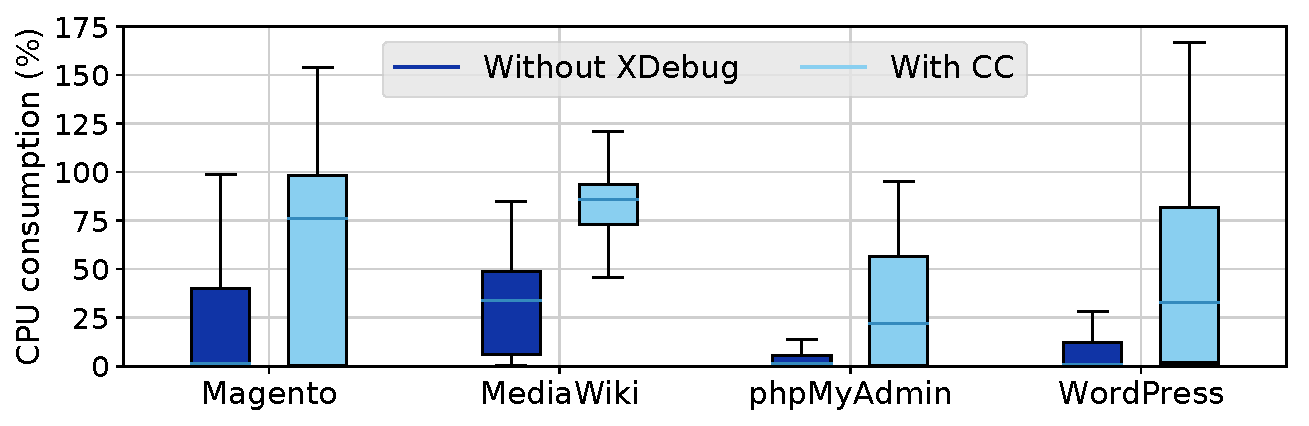
\includegraphics[width=\linewidth]{figures/cpu.pdf}
  \caption{Measurement of the CPU consumption for the tested web
  applications. 100\% corresponds to the use of a single CPU core.}
  \label{fig:cpu}
\end{figure}

Even though our results show that the overall overhead is substantial, it is
important to note that this overhead is not the overhead of the debloated
web applications. Debloated web applications do not require code-coverage
statistics and will therefore execute in the exact same environment as
the original application (i.e. without \texttt{XDebug}). Depending on how
code-coverage information is obtained, this overhead may or may not be an
issue. For example, if the coverage is calculated in an offline fashion
where traces of application usage are replayed against a testing system,
this overhead will have no impact on the real production systems. To allow
for the online computation of code coverage (using real-time user traffic),
we need more optimized code profilers. For example, \texttt{XDebug} currently
overloads 43 opcodes to obtain line-level code-coverage information that
is more fine-grained than required by our debloating techniques and incurs
an unnecessary performance overhead~\cite{xdebug-performance2}. We leave
the development and evaluation of faster code profilers for future work.

\section{Limitations}
\label{sec:limitations}
In this study, we set out to precisely quantify the security benefits of
debloating, when applied to web applications. Through a series of experiments,
we demonstrated that debloating web applications has a number of very
concrete advantages. We showed that debloating can, on average, decrease an
application's code base by removing hundreds of thousands of lines of code,
reduce its cyclomatic complexity by 30-50\% and remove code associated with
up to half of historical CVEs. Moreover, even for vulnerabilities that could
not be removed, debloating can remove gadgets that makes their exploitation
significantly harder. Next, we discuss some of the inherent and technical limitations of our approach and future direction.

\vspace{1ex}

\noindent\textbf{Lack of available exploits:} The number of exploits publicly available compared to the total number of registered CVEs is low. At the same time, the effort to study vulnerability reports, find the relevant patch or bug report, and track the actual vulnerability down to source code level takes a non-negligible amount of manual labor.
% Moreover, these public exploits usually favor certain types of vulnerabilities over others (e.g. favoring remote-command execution over XSS).
This lack of available exploits limits our ability to test the exploitability of vulnerabilities before debloating since certain vulnerabilities might only be exploitable under specific configurations.
For example the set of five file-upload-related vulnerabilities in our MediaWiki dataset (marked as gray in Table~\ref{table:listofallcves}) require access to file upload functionality which is disabled by default. A maintained set of automated, replayable exploits against popular web applications similar to ``BugBox'' introduced by Nilson et al. in 2013, could substantially help researchers at this step\cite{bugbox}.

To address this issue, we mapped the CVEs to features within those applications. This is done by studying the architecture of
target applications based on documentation within the code and available on their websites. We marked a CVE as unexploitable if the underlying feature is disabled by default, and online tutorials in our dataset do not
require users to enable that functionality. This limitation only applies to reported numbers on removed CVEs and does not affect our results on POI gadgets since their mere existence is enough for them to be used in gadget chains.

Our approach results in lower bounds for CVE removal since disabling modules through application configuration does not guarantee removal of all code paths that trigger those modules. Taking CVE-2019-6703 as an example, a vulnerability was discovered in the WordPress ``Total Donations'' plugin~\cite{wordpressPlugin} and disabling this plugin did not prevent attackers from invoking the vulnerable end point and running their exploits.

\vspace{1ex}
\noindent\textbf{Dynamic code coverage:}  Given our reliance on dynamic
code-coverage techniques, it is clear that the success of debloating a web application
is tightly related to its usage profile. Even though we constructed profiles
in a way that is reproducible and unbiased (i.e. by relying on external
popular tutorials, monkey testing, crawlers, and vulnerability scanners), we cannot claim that
real web users would not trigger code that was removed during the stage of
debloating, while they are interacting with a debloated web application.

More specifically, our modeled usage profiles do not cover all possible benign states of target web applications as we assume that users do not use all available features.
Our intuition behind debloating proves to be successful to a large degree since removing unnecessary features brings clear security improvements.
At the same time, our current usage model may not cover deep error states (e.g. logical errors in multi-stage form submissions, or the invalid structure of uploaded files).
As such, we intend to follow-up this work with crowd sourcing and user studies
to understand how administrators, developers, and regular users utilize the
evaluated web applications and whether their usage profiles would allow for
similar levels of debloating.

Due to nature of our approach, we can not take advantage of standard
static-analysis techniques, since we aim to remove the features that are
not useful for a given set of users, not those that are not reachable by
other code. Using static analysis would greatly overestimate the code that
needs to be maintained through the process of debloating and the resulting
web application would contain code (and therefore vulnerabilities) that is
not useful to all users. Going forward, we envision a hybrid approach where
dynamic analysis is used as a first step to identify the core features that
are useful for a specific set of users. These features can then be used as
a starting point for a follow-up static analysis phase to ensure that all
code related to these features is maintained when debloating a web application.

\vspace{1ex}
\noindent\textbf{Handling requests to removed code:}
A separate issue is that of handling requests to removed code. Our
current prototype utilizes assertions to log these requests so that we can
investigate why the corresponding server-side code was not captured by our
coverage profiler. When real users utilize debloated web applications,
one must decide how these failures (i.e. client-side requests requiring
server-side code that was removed) will be handled. Assuming that cleanly
exiting the application and showing an error to the user is not sufficient,
we need methods to authenticate the user's request, determine whether the
request is a benign one (and not a malicious request that aims to exploit
the debloated web application) and potentially re-introduce the removed
code. The client/server architecture of web applications lends itself well
to this model since the web server can decide to re-introduce debloated code
and handle the user's request, without any knowledge of this happening from
the side of the user. All of this, however, requires server-side systems
to introduce the code at the right time and for the appropriate users. We
leave the design of such systems for future work.

\vspace{1ex}
\noindent\textbf{Metrics to measure debloating effectiveness:}
In this paper, we use Cyclomatic Complexity (CC), Logical Lines of Code
(LLOC), reduction in historical CVEs, and POP gadget reduction as four metrics to measure the
effects of debloating on different web applications. However, not every line of code
contributes equally to a program's attack surface. For example, 15\% of removed
files from Magento 2.0.5 are test files for external packages and
the core of the application. Such code may not be directly exploitable or
used in a POP chain unless there is a misconfiguration (e.g., autoloading
including these files, or the directories being publicly accessible). As such,
the resulted reduction in source code metrics (CC and LLOC) may also reflect the code
that does not contribute to the attack surface.
Contrastingly, the reduction of exploitable CVEs draws a more realistic picture
of real world attacks. The drawback of this metric is its unavailability for
proprietary software and the manual effort required to map CVEs to source
code and verify their exploitability.

\vspace{1ex}
\noindent\textbf{Debloating effectiveness:}
Through our debloating experiments we discovered that, in terms of debloating,
not all applications are ``equal.'' Modular web applications debloat
significantly better than monolithic ones (such as Wordpress). We hope that
our findings will inspire different debloating strategies that lend themselves
better to monolithic web applications which resist our current function-level
and file-level debloating strategies.




%Finally, this study focuses on the feasibility of debloating based on usage profiles. We tried to model the behavior of general users of these applications through tutorials and other mechanisms, but production environments are vastly versatile in terms of usage of application features
%and the full potential of debloating is ultimately based on the users of instances of applications. As such, efforts to tune the performance of our system and its dependencies to their full potential
%are left for future.

\chapter{Future work}
In this section, we discuss the future directions and improvements to our current prototype that we intend to pursue in future work.

\subsection{End-to-end web application debloating}
In this work, we showed that web application debloating has the potential to significantly reduce the attack surface despite the challenges involved. Next, we discuss some of these challenges and propose directions for our future work on this topic.

\subsubsection{Handling calls to removed code}
One of the biggest challenges of using debloating in production applications is handling calls to removed functions. In our current implementation, upon executing a function that leads to debloated code, the requested operation is terminated. Then the user is notified that the intended functionality has been removed. This can happen after clicking on a link, or after several steps into filling a multi-step form. To make this more user friendly and enable website administrators to make the final decision, we envision several improvements:
\begin{itemize}

\item Adding the functionality to dynamically reintroduce the removed
code. This decision can be made either through an administration panel, or
after a second factor of authentication for privileged users. For that, we
need to identify high-risk actions and enforce further security mechanisms
and identity verification steps before continuing. From another point of
view, this step can be seen as an anomaly detection system based on history
of the user behavior.

\item Our current hypothesis is based on the observation that not all users of
an application require all features. To go one step further, one can pursue,
user-based and role-based debloating. Under this scenario, different sets of users
for the same web application are provided with their own debloated versions
based on their activity history.
\end{itemize}

\subsubsection{Propagating debloating changes to the UI}
Our current debloating setup will show error messages to users, when
they execute removed code. By disabling UI elements that exercise the
removed features we can proactively stop users from running into these
errors. Specifically, by tracking web application UI elements back to their
implementation and doing a backward traversal on the call graph, we can build
this dependency chain and disable/limit/modify UI elements. This will warn
users about the disabled features before investing any time and effort on
that function.

\begin{figure}[t]
  \centering
  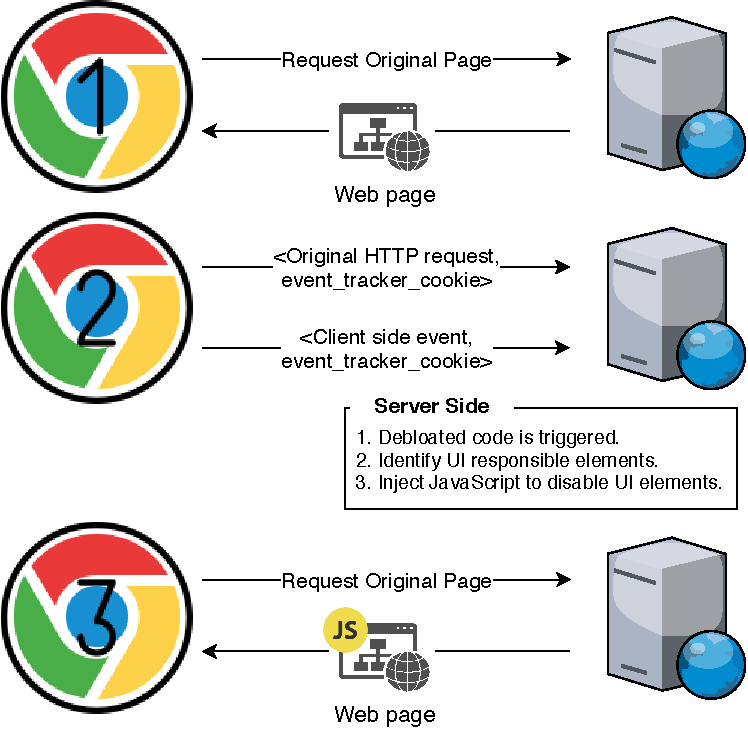
\includegraphics[width=0.7\linewidth]{figures/UI-backend-debloating.pdf}
  \caption{Overview of steps required to detect and remove UI elements for debloated actions.}
  \label{fig:uidebloating}
\end{figure}

\paragraph{Implementation details:} Web applications consist of two main components, server side and client side. Client-side code runs on users' browsers and generates HTTP requests based on user interactions with HTML and JavaScript components on the page. From server's point of view, generation of HTML content and events received from the browser are totally disconnected. The goal is to build this bridge and track server-side events as the result of client-side interactions with minimal reliance on specific application architectures.

Figure~\ref{fig:uidebloating} depicts the browser interactions required to detect and disable debloated actions on client side. Initially, PHP code is injected into all pages of the web application to add tracker cookies that are sent along page events that are reported to the server. During the first user interaction with the page at step 2 (e.g., Form submission, click on a link, etc.), by correlating the events and UI elements that triggered the request through the cookie values, we will be able to find elements and forms that trigger debloated events. The next time users request the same page, at step 3, the elements that triggered debloated actions are disabled through injected JavaScript.

\subsubsection{Code coverage collection in production environments}
By shipping the code coverage collection infrastructure to real-world users and website owners, we can gain insights into how the applications are used by different types of users.

\paragraph{Optimized code coverage collection:} To make code coverage recording less resource intensive, we need to know the source of this overhead.
Our toolset is built on top of XDebug PHP extension. To collect line level code coverage, XDebug hooks into various PHP opcodes. This makes the program execution slower and more resource intensive. Meanwhile, we only need function coverage information in our setup. This information can either be collected by a light-weight code profiler that is optimized for this task, or by developing and including PHP libraries in web applications that collect execution traces from call stack. To that end, we plan to develop optimized code profilers that can be easily installed and integrated with web applications without the need to enable PHP extensions and undergo significant performance overhead. Furthermore, by relying on function coverage instead of line coverage, our code coverage information will be more resilient to small changes that affect the order of source line numbers.

To further reduce the overhead, one can only record the code coverage for functions that include sensitive API calls (e.g., Filesystem and database interaction, dynamic code execution, network connections, etc.). The first step is to identify such functions, and through static analysis, identify code paths that interact with these APIs. By only tracking the code coverage on these specific functions, we can still reap the benefit of debloating without the associated high overheads of existing code profilers.

\subsubsection{Attack surface reduction through API specialization}
In the context of web application security, Runtime Application Self Protection (RASP) is a suite of tools and techniques that has been increasing in popularity in the recent years. By adding a defensive layer that detects attacks from within the application, the protection engine has access to execution context. This extra information increases the precision of the protection engine in detecting attacks.

A similar idea can be applied to debloating web applications. When normal users interact with a web application, functions and APIs are invoked with specific sets of parameters. By dynamically generating and enforcing whitelists that only allow benign invocation of security critical APIs, we can block exploitation attempts and reduce the attack surface and exploitability of our software.

As a motivating example, we look at the following SQL injection vulnerability in AutoSuggest 0.24 WordPress plugin~\cite{autosuggest_vulnerability}:

\begin{figure}[t]
\begin{lstlisting}[frame=single, caption={PHP code from AutoSuggest WordPress plugin with SQL injection vulnerability},captionpos=b, label={listing:autosuggest_sqli}]
<?php
$wpas_keys = $_GET['wpas_keys'];
$pageposts = $wpdb->get_results("SELECT * FROM $wpdb->posts
WHERE (post_title LIKE '%$wpas_keys%') AND post_status = 'publish' ORDER BY post_date DESC");
\end{lstlisting}
\end{figure}

Benign queries in Listing~\ref{listing:autosuggest_sqli} only target \$wpdb.posts table, whereas an exploit will likely target other tables via subqueries and UNION and try to access users table and extract information. Notice that \$wpdb.posts variable comes from WordPress configuration file and is static for each installation of WordPress.
By running each query under a different user that has the minimal permissions that satisfy the benign invocations of target query (e.g., by limiting the target table for a given query), the exploit attempt will fail.
So in this example, the query would run under the automatically generated user named ``wp\_posts\_user'' which only has ``SELECT'' permission to WordPress ``posts'' table. This would limit the exploit to be able to extract information only from posts table.

To implement this idea, we would start by creating a list of security critical PHP functions.
For each critical API, we distinguish benign and malicious invocations at runtime by learning from application usage and create a whitelist that is dynamically generated and enforces conditions to minimize the set of possible invocations of these APIs.

More concretely, we distinguish the following cases:
\begin{itemize}
  \item \textbf{Database Operations:} In the context of database operations, we limit type of operation (e.g., SELECT query) and target tables (e.g., Posts table) and database (WordPress db) for each database interaction. This can be implemented as a proxy between the database and the application or by modifying the database layer within the application (e.g., modifying the ORM). This modified API should dynamically learn and decide how the api is called and what rules should be enforced.
  \item \textbf{File System Interactions:} For these APIs, we enforce target directories, allowed file extensions and their permissions. For example, if the code writes to the file system, we dynamically learn the target directory and type/permission of files submitted through this API.
  Another possible variation is to mount virtual directories that are not directly accessible from the web, but are accessible by the PHP code itself. This prevents uploading a PHP backdoor and executing it directly from the web.
  \item \textbf{Limiting Available APIs:} By limiting the set of PHP APIs that are available to each PHP file, we can block potential exploits. For example, the login.php file should not interact with the file system or call ``eval'' or ``exec''.
\end{itemize}

\section{Conclusion}
In this project, we analyzed the impact of removing unnecessary code in modern
web applications through a process called \textit{software debloating}.
We presented the pipeline details of the end-to-end, modular debloating
framework that we designed and implemented, allowing us to record how a
PHP application is used and what server-side code is triggered as a result of
client-side requests. After retrieving code-coverage information, our debloating
framework removes unused parts of
an application using file-level and function-level debloating.

By evaluating
our framework on four popular PHP applications (phpMyAdmin, MediaWiki,
Magento, and WordPress) we witnessed the clear security benefits of debloating web
applications. We observed a significant LLOC decrease ranging between
9\% to 64\% for file-level debloating and up to an additional 24\% with
function-level debloating. Next, we showed that external packages are one
of the primary source of bloat as our debloating framework was able to remove
more than 84\% of unused code in versions that used Composer, PHP's most popular
package manager. By quantifying the removal of code associated with critical
CVEs, we observed a reduction of up to 60\% of high-impact, historical vulnerabilities.
Finally, we showed that the process of debloating also removes
instructions and classes that are the primary sources for attackers to build
gadgets and perform POI attacks.

Our results demonstrate that debloating web applications
provides tangible security benefits and therefore should be seriously
considered as a practical way of reducing the attack surface of
web-applications deployments.


\chapter{Future work}
In this section, we discuss the future directions and improvements to our current prototype that we intend to pursue in future work.

\subsection{End-to-end web application debloating}
In this work, we showed that web application debloating has the potential to significantly reduce the attack surface despite the challenges involved. Next, we discuss some of these challenges and propose directions for our future work on this topic.

\subsubsection{Handling calls to removed code}
One of the biggest challenges of using debloating in production applications is handling calls to removed functions. In our current implementation, upon executing a function that leads to debloated code, the requested operation is terminated. Then the user is notified that the intended functionality has been removed. This can happen after clicking on a link, or after several steps into filling a multi-step form. To make this more user friendly and enable website administrators to make the final decision, we envision several improvements:
\begin{itemize}

\item Adding the functionality to dynamically reintroduce the removed
code. This decision can be made either through an administration panel, or
after a second factor of authentication for privileged users. For that, we
need to identify high-risk actions and enforce further security mechanisms
and identity verification steps before continuing. From another point of
view, this step can be seen as an anomaly detection system based on history
of the user behavior.

\item Our current hypothesis is based on the observation that not all users of
an application require all features. To go one step further, one can pursue,
user-based and role-based debloating. Under this scenario, different sets of users
for the same web application are provided with their own debloated versions
based on their activity history.
\end{itemize}

\subsubsection{Propagating debloating changes to the UI}
Our current debloating setup will show error messages to users, when
they execute removed code. By disabling UI elements that exercise the
removed features we can proactively stop users from running into these
errors. Specifically, by tracking web application UI elements back to their
implementation and doing a backward traversal on the call graph, we can build
this dependency chain and disable/limit/modify UI elements. This will warn
users about the disabled features before investing any time and effort on
that function.

\begin{figure}[t]
  \centering
  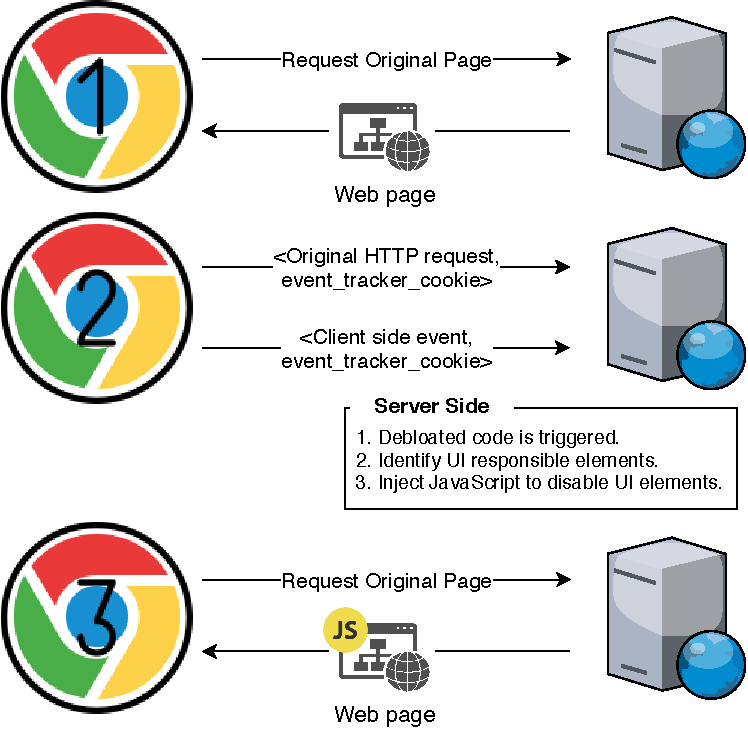
\includegraphics[width=0.7\linewidth]{figures/UI-backend-debloating.pdf}
  \caption{Overview of steps required to detect and remove UI elements for debloated actions.}
  \label{fig:uidebloating}
\end{figure}

\paragraph{Implementation details:} Web applications consist of two main components, server side and client side. Client-side code runs on users' browsers and generates HTTP requests based on user interactions with HTML and JavaScript components on the page. From server's point of view, generation of HTML content and events received from the browser are totally disconnected. The goal is to build this bridge and track server-side events as the result of client-side interactions with minimal reliance on specific application architectures.

Figure~\ref{fig:uidebloating} depicts the browser interactions required to detect and disable debloated actions on client side. Initially, PHP code is injected into all pages of the web application to add tracker cookies that are sent along page events that are reported to the server. During the first user interaction with the page at step 2 (e.g., Form submission, click on a link, etc.), by correlating the events and UI elements that triggered the request through the cookie values, we will be able to find elements and forms that trigger debloated events. The next time users request the same page, at step 3, the elements that triggered debloated actions are disabled through injected JavaScript.

\subsubsection{Code coverage collection in production environments}
By shipping the code coverage collection infrastructure to real-world users and website owners, we can gain insights into how the applications are used by different types of users.

\paragraph{Optimized code coverage collection:} To make code coverage recording less resource intensive, we need to know the source of this overhead.
Our toolset is built on top of XDebug PHP extension. To collect line level code coverage, XDebug hooks into various PHP opcodes. This makes the program execution slower and more resource intensive. Meanwhile, we only need function coverage information in our setup. This information can either be collected by a light-weight code profiler that is optimized for this task, or by developing and including PHP libraries in web applications that collect execution traces from call stack. To that end, we plan to develop optimized code profilers that can be easily installed and integrated with web applications without the need to enable PHP extensions and undergo significant performance overhead. Furthermore, by relying on function coverage instead of line coverage, our code coverage information will be more resilient to small changes that affect the order of source line numbers.

To further reduce the overhead, one can only record the code coverage for functions that include sensitive API calls (e.g., Filesystem and database interaction, dynamic code execution, network connections, etc.). The first step is to identify such functions, and through static analysis, identify code paths that interact with these APIs. By only tracking the code coverage on these specific functions, we can still reap the benefit of debloating without the associated high overheads of existing code profilers.

\subsubsection{Attack surface reduction through API specialization}
In the context of web application security, Runtime Application Self Protection (RASP) is a suite of tools and techniques that has been increasing in popularity in the recent years. By adding a defensive layer that detects attacks from within the application, the protection engine has access to execution context. This extra information increases the precision of the protection engine in detecting attacks.

A similar idea can be applied to debloating web applications. When normal users interact with a web application, functions and APIs are invoked with specific sets of parameters. By dynamically generating and enforcing whitelists that only allow benign invocation of security critical APIs, we can block exploitation attempts and reduce the attack surface and exploitability of our software.

As a motivating example, we look at the following SQL injection vulnerability in AutoSuggest 0.24 WordPress plugin~\cite{autosuggest_vulnerability}:

\begin{figure}[t]
\begin{lstlisting}[frame=single, caption={PHP code from AutoSuggest WordPress plugin with SQL injection vulnerability},captionpos=b, label={listing:autosuggest_sqli}]
<?php
$wpas_keys = $_GET['wpas_keys'];
$pageposts = $wpdb->get_results("SELECT * FROM $wpdb->posts
WHERE (post_title LIKE '%$wpas_keys%') AND post_status = 'publish' ORDER BY post_date DESC");
\end{lstlisting}
\end{figure}

Benign queries in Listing~\ref{listing:autosuggest_sqli} only target \$wpdb.posts table, whereas an exploit will likely target other tables via subqueries and UNION and try to access users table and extract information. Notice that \$wpdb.posts variable comes from WordPress configuration file and is static for each installation of WordPress.
By running each query under a different user that has the minimal permissions that satisfy the benign invocations of target query (e.g., by limiting the target table for a given query), the exploit attempt will fail.
So in this example, the query would run under the automatically generated user named ``wp\_posts\_user'' which only has ``SELECT'' permission to WordPress ``posts'' table. This would limit the exploit to be able to extract information only from posts table.

To implement this idea, we would start by creating a list of security critical PHP functions.
For each critical API, we distinguish benign and malicious invocations at runtime by learning from application usage and create a whitelist that is dynamically generated and enforces conditions to minimize the set of possible invocations of these APIs.

More concretely, we distinguish the following cases:
\begin{itemize}
  \item \textbf{Database Operations:} In the context of database operations, we limit type of operation (e.g., SELECT query) and target tables (e.g., Posts table) and database (WordPress db) for each database interaction. This can be implemented as a proxy between the database and the application or by modifying the database layer within the application (e.g., modifying the ORM). This modified API should dynamically learn and decide how the api is called and what rules should be enforced.
  \item \textbf{File System Interactions:} For these APIs, we enforce target directories, allowed file extensions and their permissions. For example, if the code writes to the file system, we dynamically learn the target directory and type/permission of files submitted through this API.
  Another possible variation is to mount virtual directories that are not directly accessible from the web, but are accessible by the PHP code itself. This prevents uploading a PHP backdoor and executing it directly from the web.
  \item \textbf{Limiting Available APIs:} By limiting the set of PHP APIs that are available to each PHP file, we can block potential exploits. For example, the login.php file should not interact with the file system or call ``eval'' or ``exec''.
\end{itemize}

\section{Conclusion}
In this project, we analyzed the impact of removing unnecessary code in modern
web applications through a process called \textit{software debloating}.
We presented the pipeline details of the end-to-end, modular debloating
framework that we designed and implemented, allowing us to record how a
PHP application is used and what server-side code is triggered as a result of
client-side requests. After retrieving code-coverage information, our debloating
framework removes unused parts of
an application using file-level and function-level debloating.

By evaluating
our framework on four popular PHP applications (phpMyAdmin, MediaWiki,
Magento, and WordPress) we witnessed the clear security benefits of debloating web
applications. We observed a significant LLOC decrease ranging between
9\% to 64\% for file-level debloating and up to an additional 24\% with
function-level debloating. Next, we showed that external packages are one
of the primary source of bloat as our debloating framework was able to remove
more than 84\% of unused code in versions that used Composer, PHP's most popular
package manager. By quantifying the removal of code associated with critical
CVEs, we observed a reduction of up to 60\% of high-impact, historical vulnerabilities.
Finally, we showed that the process of debloating also removes
instructions and classes that are the primary sources for attackers to build
gadgets and perform POI attacks.

Our results demonstrate that debloating web applications
provides tangible security benefits and therefore should be seriously
considered as a practical way of reducing the attack surface of
web-applications deployments.

\appendix % all chapters following will be labeled as appendices
\begin{table}[]
\centering
\caption{Comprehensive list of mapped CVEs and whether vulnerable files, functions or lines were triggered based on our usage profiles. Grey rows indicate CVEs located in modules that are, by default, disabled.}
\label{table:listofallcves}
\scalebox{0.53}{
\begin{tabular}{|l|l|l|c|c|c|l|}
\hline
\multicolumn{7}{|c|}{\textbf{phpMyAdmin}} \\
\hline
\multirow{2}{*}{\textbf{\#}}     & \multicolumn{1}{c|}{\multirow{2}{*}{\textbf{CVE}}} & \multicolumn{1}{c|}{\multirow{2}{*}{\textbf{Ver.}}}            & \multicolumn{3}{c|}{\textbf{Vulnerability Triggered}}                                 & \multicolumn{1}{c|}{\multirow{2}{*}{\textbf{Affected Functionality}}} \\ \cline{4-6}
                        & \multicolumn{1}{c|}{}                     & \multicolumn{1}{c|}{}                & \textbf{Files}                         & \textbf{Functions}                     & \textbf{Lines}                         & \multicolumn{1}{c|}{}                                        \\ \hline
1                       & CVE-2013-3238                             &  4.0.0                               & \faCheck                      & NA                            & \faTimes                      & Rename table using Regex                                     \\ \hline
2                       & CVE-2013-3240                             &  4.0.0                               & \faCheck                      & \faCheck                      & \faCheck                      & Plugins                                                      \\ \hline
3                       & CVE-2014-8959                             &  4.0.0                               & \faTimes                      & \faTimes                      & \faTimes                      & GIS Editor                                                   \\ \hline
4                       & CVE-2016-6609                             &  4.0.0                               & \faCheck                      & \faTimes                      & \faTimes                      & Export as phparray                                           \\ \hline
5                       & CVE-2016-6619                             &  4.0.0                               & \faCheck                      & \faTimes                      & \faTimes                      & Recent tables                                                \\ \hline
\rowcolor{lightgray}6   & CVE-2016-6620                             &  4.0.0                               & \faTimes                      & \faTimes                      & \faTimes                      & Table tracking                                               \\ \hline
7                       & CVE-2016-6628                             &  4.0.0                               & \faTimes                      & \faTimes                      & \faTimes                      & Create charts                                                \\ \hline
8                       & CVE-2016-6629                             &  4.0.0                               & \faTimes                      & \faTimes                      & \faTimes                      & Configuration option                                         \\ \hline
9                       & CVE-2016-6631                             &  4.0.0                               & \faTimes                      & \faTimes                      & \faTimes                      & Create transform plugins                                     \\ \hline
10                      & CVE-2016-6633                             &  4.0.0                               & \faCheck                      & \faTimes                      & \faTimes                      & Import ESRI shape file                                       \\ \hline
11                      & CVE-2016-9866                             &  4.0.0                               & \faCheck                      & NA                            & \faTimes                      & User preferences                                             \\ \hline
12                      & CVE-2016-5703                             &  4.4.0                               & \faCheck                      & \faTimes                      & \faTimes                      & Central columns                                              \\ \hline
13                      & CVE-2016-5734                             &  4.4.0                               & \faCheck                      & \faTimes                      & \faTimes                      & Table search using Regex                                     \\ \hline
14                      & CVE-2016-6616                             &  4.4.0                               & \faTimes                      & \faTimes                      & \faTimes                      & User groups                                                  \\ \hline
15                      & CVE-2017-1000017                          &  4.4.0                               & \faCheck                      & \faCheck                      & \faTimes                      & Replication                                                  \\ \hline
16                      & CVE-2016-6606                             &  4.6.0                               & \faCheck                      & \faCheck                      & \faCheck                      & Authentication cookies                                       \\ \hline
17                      & CVE-2016-6617                             &  4.6.0                               & \faCheck                      & \faTimes                      & \faTimes                      & Export templates                                             \\ \hline
18                      & CVE-2016-9849                             &  4.6.0                               & \faCheck                      & \faCheck                      & \faCheck                      & Authentication                                               \\ \hline
19                      & CVE-2016-9865                             &  4.6.0                               & \faCheck                      & NA                            & \faTimes                      & Core deserialization                                         \\ \hline
20                      & CVE-2017-1000499                          &  4.7.0                               & \faCheck                      & \faCheck                      & \faCheck                      & Navigation tree                                              \\ \hline
\multicolumn{7}{|c|}{\textbf{MediaWiki}} \\ \hline
\rowcolor{lightgray}21  & CVE-2013-2114                             &  1.19.1                              & \faCheck                      & \faTimes                      & \faTimes                      & File upload from chunks                                      \\ \hline
\rowcolor{lightgray}22  & CVE-2013-6453                             &  1.21.1                              & \faCheck                      & \faTimes                      & \faTimes                      & Verify uploaded file                                         \\ \hline
\rowcolor{lightgray}23  & CVE-2014-1610                             &  1.21.1                              & \faCheck                      & \faTimes                      & \faTimes                      & PDF Upload                                                   \\ \hline
24                      & CVE-2014-2243                             &  1.21.1                              & \faCheck                      & \faCheck                      & \faTimes                      & User settings                                                \\ \hline
25                      & CVE-2014-5241                             &  1.21.1                              & \faCheck                      & \faTimes                      & \faTimes                      & JSON Output formatter                                        \\ \hline
26                      & CVE-2014-9277                             &  1.21.1                              & \faCheck                      & \faTimes                      & \faTimes                      & Flash policy output                                          \\ \hline
27                      & CVE-2014-9276                             &  1.23.0                              & \faCheck                      & \faCheck                      & \faCheck                      & Expand templates                                             \\ \hline
28                      & CVE-2015-2936                             &  1.24.0                              & \faCheck                      & \faCheck                      & \faCheck                      & Authentication                                               \\ \hline
29                      & CVE-2015-2937                             &  1.24.0                              & \faTimes                      & \faTimes                      & \faTimes                      & XMP data reader                                              \\ \hline
30                      & CVE-2015-6728                             &  1.24.0                              & \faCheck                      & \faTimes                      & \faTimes                      & Get watchlists through API                                   \\ \hline
\rowcolor{lightgray}31  & CVE-2015-8002                             &  1.24.0                              & \faCheck                      & \faTimes                      & \faTimes                      & File upload from chunks                                      \\ \hline
\rowcolor{lightgray}32  & CVE-2015-8003                             &  1.24.0                              & \faCheck                      & \faTimes                      & \faTimes                      & File upload API                                              \\ \hline
33                      & CVE-2015-8623                             &  1.24.0                              & \faTimes                      & \faTimes                      & \faTimes                      & User object                                                  \\ \hline
34                      & CVE-2015-8624                             &  1.24.0                              & \faTimes                      & \faTimes                      & \faTimes                      & User object                                                  \\ \hline
35                      & CVE-2017-0370                             &  1.24.0                              & \faCheck                      & \faCheck                      & \faCheck                      & Markup parser (blacklist)                                    \\ \hline
36                      & CVE-2017-0362                             &  1.28.0                              & \faCheck                      & \faCheck                      & \faCheck                      & Track pages                                                  \\ \hline
37                      & CVE-2017-0363                             &  1.28.0                              & \faCheck                      & \faCheck                      & \faCheck                      & Search                                                       \\ \hline
38                      & CVE-2017-0364                             &  1.28.0                              & \faCheck                      & \faCheck                      & \faCheck                      & Search                                                       \\ \hline
39                      & CVE-2017-0367                             &  1.28.0                              & \faCheck                      & \faCheck                      & \faCheck                      & Localization cache                                           \\ \hline
40                      & CVE-2017-0368                             &  1.28.0                              & \faCheck                      & \faCheck                      & \faCheck                      & System messages                                              \\ \hline
41                      & CVE-2017-8809                             &  1.28.0                              & \faCheck                      & \faCheck                      & \faCheck                      & APIs and RSS                                                 \\ \hline
\multicolumn{7}{|c|}{\textbf{Magento}} \\ \hline
42                      & CVE-2015-1397                             & 1.9.0                                & \faCheck                      & \faCheck                      & \faCheck                      & Prepare SQL condition                                        \\ \hline
43                      & CVE-2015-1398                             & 1.9.0                                & \faCheck                      & \faCheck                      & \faTimes                      & OAuth \& XML modules                                         \\ \hline
44                      & CVE-2015-1399                             & 1.9.0                                & \faCheck                      & \faCheck                      & \faCheck                      & Actions predispatch                                          \\ \hline
45                      & CVE-2015-8707                             & 1.9.0                                & \faCheck                      & \faTimes                      & \faTimes                      & Password reset                                               \\ \hline
46                      & CVE-2016-2212                             & 1.9.0                                & \faCheck                      & \faTimes                      & \faTimes                      & Order status RSS                                             \\ \hline
47                      & CVE-2016-4010                             & 2.0.5                                & \faCheck                      & \faCheck                      & \faCheck                      & Shopping cart                                                \\ \hline
48                      & CVE-2016-6485                             & 2.0.5                                & \faCheck                      & \faCheck                      & \faCheck                      & Cryptography functions                                       \\ \hline
49                      & CVE-2018-5301                             & 2.0.5                                & \faTimes                      & \faTimes                      & \faTimes                      & Delete customer address                                      \\ \hline
\multicolumn{7}{|c|}{\textbf{WordPress}} \\ \hline
50                      & CVE-2014-5203                             & 3.9                                  & \faCheck                      & \faCheck                      & \faTimes                      & Widget customization                                         \\ \hline
51                      & CVE-2014-5204                             & 3.9                                  & \faCheck                      & \faCheck                      & \faCheck                      & CSRF token verification                                      \\ \hline
52                      & CVE-2014-5205                             & 3.9                                  & \faCheck                      & \faCheck                      & \faCheck                      & CSRF token verification                                      \\ \hline
53                      & CVE-2018-12895                            & 3.9                                  & \faCheck                      & \faCheck                      & \faCheck                      & Delete post thumbnail                                        \\ \hline
54                      & CVE-2015-2213                             & 4.0                                  & \faCheck                      & \faCheck                      & \faCheck                      & Untrash comment                                              \\ \hline
55                      & CVE-2017-14723                            & 4.0                                  & \faCheck                      & \faCheck                      & \faCheck                      & Prepared queries                                             \\ \hline
56                      & CVE-2014-9033                             & 4.0                                  & \faCheck                      & \faCheck                      & \faTimes                      & Password reset                                               \\ \hline
57                      & CVE-2014-9037                             & 4.0                                  & \faCheck                      & \faCheck                      & \faCheck                      & Password hashing library                                     \\ \hline
58                      & CVE-2016-6635                             & 4.0                                  & \faCheck                      & \faTimes                      & \faTimes                      & Ajax compression test                                        \\ \hline
59                      & CVE-2014-9038                             & 4.0                                  & \faCheck                      & \faCheck                      & \faCheck                      & HTTP request API                                             \\ \hline
60                      & CVE-2015-5731                             & 4.2.3                                & \faCheck                      & \faCheck                      & \faTimes                      & Admin panel                                                  \\ \hline
61                      & CVE-2016-7169                             & 4.6                                  & \faCheck                      & \faCheck                      & \faTimes                      & Sanitize uploaded file name                                  \\ \hline
62                      & CVE-2017-17091                            & 4.6                                  & \faCheck                      & NA                            & \faTimes                      & Create new user                                              \\ \hline
63                      & CVE-2017-5492                             & 4.7                                  & \faCheck                      & \faCheck                      & \faCheck                      & Admin screen API, widgets                                    \\ \hline
64                      & CVE-2017-9064                             & 4.7                                  & \faCheck                      & \faCheck                      & \faCheck                      & Admin file system operations                                 \\ \hline
65                      & CVE-2018-10101                            & 4.7                                  & \faCheck                      & \faCheck                      & \faCheck                      & HTTP request API                                             \\ \hline
66                      & CVE-2018-10100                            & 4.7                                  & \faCheck                      & NA                            & \faTimes                      & Login                                                        \\ \hline
67                      & CVE-2017-6815                             & 4.7                                  & \faCheck                      & \faCheck                      & \faCheck                      & Redirect URL validation                                      \\ \hline
68                      & CVE-2017-5611                             & 4.7.1                                & \faCheck                      & \faCheck                      & \faCheck                      & Query helper                                                 \\ \hline
69                      & CVE-2017-16510                            & 4.7.1                                & \faCheck                      & \faTimes                      & \faTimes                      & Prepared queries                                             \\ \hline
\end{tabular}
}
\end{table}


%\begin{table}[]
%  \footnotesize
%  \centering
%\caption{Comprehensive list of tutorials collected from the first two pages of Google search results}
%\label{table:listoftutorials}
%\begin{tabular}{|l|p{7.3cm}|}
%\hline
%\multicolumn{2}{|c|}{\textbf{phpMyAdmin}}  \\ \hline
%  \href{https://web.archive.org/web/20181112232555/https://www.siteground.com/tutorials/phpmyadmin/}{A}                                                             & \href{https://www.siteground.com/tutorials/phpmyadmin/}{https://www.siteground.com/tutorials/phpmyadmin/}                                    \\ \hline
%  \href{https://web.archive.org/web/20181112233149/https://www.reg.ca/faq/PhpMyAdminTutorial.html}{A}                                                               & \href{https://www.reg.ca/faq/PhpMyAdminTutorial.html}{https://www.reg.ca/faq/PhpMyAdminTutorial.html} \\ \hline
%  \href{https://web.archive.org/web/20181114201249/https://www.w3resource.com/mysql/administration-tools/phpmyadmin-tutorial.php}{A}                                & \href{https://www.w3resource.com/mysql/administration-tools/phpmyadmin-tutorial.php}{https://www.w3resource.com/mysql/administration-tools/phpmyadmin-tutorial.php} \\ \hline
%  \href{https://web.archive.org/web/20181112233311/https://code.tutsplus.com/tutorials/installing-and-using-phpmyadmin-for-web-development--cms-21947}{A}           & \href{https://code.tutsplus.com/tutorials/installing-and-using-phpmyadmin-for-web-development--cms-21947}{https://code.tutsplus.com/tutorials/installing-and-using-phpmyadmin-for-web-development--cms-21947} \\ \hline
%  \href{https://web.archive.org/web/20181112233410/https://www.homeandlearn.co.uk/php/php12p2.html}{A}                                                              & \href{https://www.homeandlearn.co.uk/php/php12p2.html}{https://www.homeandlearn.co.uk/php/php12p2.html} \\ \hline
%  \href{https://web.archive.org/web/20181112233639/https://www.wpbeginner.com/beginners-guide/beginners-guide-to-wordpress-database-management-with-phpmyadmin/}{A} & \href{https://www.wpbeginner.com/beginners-guide/beginners-guide-to-wordpress-database-management-with-phpmyadmin/}{https://www.wpbeginner.com/beginners-guide/beginners-guide-to-wordpress-database-management-with-phpmyadmin/} \\ \hline
%  \href{https://web.archive.org/web/20181112233730/http://members.ipage.com/knowledgebase/read_article.bml?kbid=5923}{A}                                            & \href{http://members.ipage.com/knowledgebase/read_article.bml?kbid=5923}{http://members.ipage.com/knowledgebase/read\_article.bml?kbid=5923} \\ \hline
%  \href{https://web.archive.org/web/20181112233831/https://www.digitalocean.com/community/tutorials/how-to-install-and-secure-phpmyadmin-on-ubuntu-16-04}{A}        & \href{https://www.digitalocean.com/community/tutorials/how-to-install-and-secure-phpmyadmin-on-ubuntu-16-04}{https://www.digitalocean.com/community/tutorials/how-to-install-and-secure-phpmyadmin-on-ubuntu-16-04} \\ \hline
%  \href{https://web.archive.org/web/20181112233904/https://www.fastwebhost.com/tutorials/knowledge-base/phpmyadmin-tutorial-administration-2/}{A}                   & \href{https://www.fastwebhost.com/tutorials/knowledge-base/phpmyadmin-tutorial-administration-2/}{https://www.fastwebhost.com/tutorials/knowledge-base/phpmyadmin-tutorial-administration-2/} \\ \hline
%  \href{https://web.archive.org/web/20181112234156/https://www.tutorialspoint.com/cpanel/cpanel_phpmyadmin.htm}{A}                                                  & \href{https://www.tutorialspoint.com/cpanel/cpanel_phpmyadmin.htm}{https://www.tutorialspoint.com/cpanel/cpanel\_phpmyadmin.htm} \\ \hline
%  \href{https://web.archive.org/web/20181112234218/https://www.w3schools.com/php/php_mysql_intro.asp}{A}                                                            & \href{https://www.w3schools.com/php/php_mysql_intro.asp}{https://www.w3schools.com/php/php\_mysql\_intro.asp} \\ \hline
%  \href{https://web.archive.org/web/20181112234543/https://pimylifeup.com/raspberry-pi-mysql-phpmyadmin/}{A}                                                        & \href{https://pimylifeup.com/raspberry-pi-mysql-phpmyadmin/}{https://pimylifeup.com/raspberry-pi-mysql-phpmyadmin/} \\ \hline
%  \href{https://web.archive.org/web/20181112234617/https://www.webhostface.com/kb/knowledgebase/mysql-search-replace/}{A}                                           & \href{https://www.webhostface.com/kb/knowledgebase/mysql-search-replace/}{https://www.webhostface.com/kb/knowledgebase/mysql-search-replace/} \\ \hline
%  \href{https://web.archive.org/web/20181112234658/https://www.eukhost.com/web-hosting/phpmyadmin.php}{A}                                                           & \href{https://www.eukhost.com/web-hosting/phpmyadmin.php}{https://www.eukhost.com/web-hosting/phpmyadmin.php} \\ \hline
%\multicolumn{2}{|c|}{\textbf{MediaWiki}}  \\ \hline
%  \href{https://web.archive.org/web/20181112234835/https://www.siteground.com/tutorials/mediawiki/}{A}                                                              & \href{https://www.siteground.com/tutorials/mediawiki/}{https://www.siteground.com/tutorials/mediawiki/}                  \\ \hline
%  \href{https://web.archive.org/web/20181112234857/http://helpwiki.evergreen.edu/wiki/index.php/Mediawiki_Tutorial}{A}                                              & \href{http://helpwiki.evergreen.edu/wiki/index.php/Mediawiki_Tutorial}{http://helpwiki.evergreen.edu/wiki/index.php/Mediawiki\_Tutorial}\\ \hline
%  \href{https://web.archive.org/web/20181112234914/https://lifehacker.com/5396832/customize-mediawiki-into-your-ultimate-collaborative-web-site}{A}                 & \href{https://lifehacker.com/5396832/customize-mediawiki-into-your-ultimate-collaborative-web-site}{https://lifehacker.com/5396832/customize-mediawiki-into-your-ultimate-collaborative-web-site} \\ \hline
%  \href{https://web.archive.org/web/20181112234947/https://hepmdb.soton.ac.uk/wiki/images/0/0b/Open4a-Getting-Started-with-mediawiki.pdf}{A}                        & \href{https://hepmdb.soton.ac.uk/wiki/images/0/0b/Open4a-Getting-Started-with-mediawiki.pdf}{https://hepmdb.soton.ac.uk/wiki/images/0/0b/Open4a-Getting-Started-with-mediawiki.pdf} \\ \hline
%  \href{https://web.archive.org/web/20181112235106/https://www.fastwebhost.com/tutorials/cat/mediawiki-tutorial/}{A}                                                & \href{https://www.fastwebhost.com/tutorials/cat/mediawiki-tutorial/}{https://www.fastwebhost.com/tutorials/cat/mediawiki-tutorial/} \\ \hline
%  \href{https://web.archive.org/web/20181112235233/https://www.semantic-mediawiki.org/wiki/Help:Getting_started}{A}                                                 & \href{https://www.semantic-mediawiki.org/wiki/Help:Getting_started}{https://www.semantic-mediawiki.org/wiki/Help:Getting\_started} \\ \hline
%  \href{https://web.archive.org/web/20181112235352/https://www.inmotionhosting.com/support/edu/mediawiki/getting-started-mediawiki}{A}                              & \href{https://www.inmotionhosting.com/support/edu/mediawiki/getting-started-mediawiki}{https://www.inmotionhosting.com/support/edu/mediawiki/getting-started-mediawiki} \\ \hline
%  \href{https://web.archive.org/web/20181112235422/https://www.hostknox.com/tutorials/mediawiki/installation}{A}                                                    & \href{https://www.hostknox.com/tutorials/mediawiki/installation}{https://www.hostknox.com/tutorials/mediawiki/installation} \\ \hline
%  \href{https://web.archive.org/web/20181112235447/https://www.digitalocean.com/community/tutorials/how-to-install-mediawiki-on-ubuntu-14-04}{A}                    & \href{https://www.digitalocean.com/community/tutorials/how-to-install-mediawiki-on-ubuntu-14-04}{https://www.digitalocean.com/community/tutorials/how-to-install-mediawiki-on-ubuntu-14-04} \\ \hline
%  \href{https://web.archive.org/web/20181112235514/https://computers.tutsplus.com/tutorials/how-to-build-your-own-wiki--cms-19772}{A}                               & \href{https://computers.tutsplus.com/tutorials/how-to-build-your-own-wiki--cms-19772}{https://computers.tutsplus.com/tutorials/how-to-build-your-own-wiki--cms-19772} \\ \hline
%  \href{https://web.archive.org/web/20181112235536/https://www.tmdhosting.com/tutorials/mediawiki/how-to-backup-mediawiki.html}{A}                                  & \href{https://www.tmdhosting.com/tutorials/mediawiki/how-to-backup-mediawiki.html}{https://www.tmdhosting.com/tutorials/mediawiki/how-to-backup-mediawiki.html}                                     \\ \hline
%\multicolumn{2}{|c|}{\textbf{Magento}}  \\ \hline
%  \href{https://web.archive.org/web/20181113025812/https://www.tutorialspoint.com/magento/}{A}                                                                      & \href{https://www.tutorialspoint.com/magento/}{https://www.tutorialspoint.com/magento/}                                                                         \\ \hline
%  \href{https://web.archive.org/web/20181113025840/https://www.siteground.com/tutorials/magento/}{A}                                                                & \href{https://www.siteground.com/tutorials/magento/}{https://www.siteground.com/tutorials/magento/} \\ \hline                                                                                                                                                              \href{https://web.archive.org/web/20181120140129/https://blog.magestore.com/magento-tutorial/}{A}                                                                & \href{https://blog.magestore.com/magento-tutorial/}{https://blog.magestore.com/magento-tutorial/}                                                                   \\ \hline
%  \href{https://web.archive.org/web/20181114201450/https://www.cminds.com/the-ultimate-beginners-guide-to-magento/}{A}                                              & \href{https://www.cminds.com/the-ultimate-beginners-guide-to-magento/}{https://www.cminds.com/the-ultimate-beginners-guide-to-magento/} \\ \hline
%  \href{https://web.archive.org/web/20181113030038/https://code.tutsplus.com/articles/from-beginner-to-advanced-in-magento-introduction-installation--cms-21969}{A} & \href{https://code.tutsplus.com/articles/from-beginner-to-advanced-in-magento-introduction-installation--cms-21969}{https://code.tutsplus.com/articles/from-beginner-to-advanced-in-magento-introduction-installation--cms-21969} \\ \hline
%  \href{https://web.archive.org/web/20181113030108/https://www.simicart.com/blog/best-magento-tutorial-resources-beginner/}{A}                                      & \href{https://www.simicart.com/blog/best-magento-tutorial-resources-beginner/}{https://www.simicart.com/blog/best-magento-tutorial-resources-beginner/} \\ \hline
%  \href{https://web.archive.org/web/20181113030148/https://www.cloudways.com/blog/magento/}{A}                                                                      & \href{https://www.cloudways.com/blog/magento/}{https://www.cloudways.com/blog/magento/} \\ \hline
%  \href{https://web.archive.org/web/20181113030232/https://magenticians.com/}{A}                                                                                    & \href{https://magenticians.com/}{https://magenticians.com/} \\ \hline
%  \href{https://web.archive.org/web/20181113030303/https://www.mageplaza.com/kb/magento-2-tutorial/}{A}                                                             & \href{https://www.mageplaza.com/kb/magento-2-tutorial/}{https://www.mageplaza.com/kb/magento-2-tutorial/} \\ \hline
%  \href{https://web.archive.org/web/20181113030342/https://devdocs.magento.com/guides/m1x/magefordev/mage-for-dev-1.html}{A}                                        & \href{https://devdocs.magento.com/guides/m1x/magefordev/mage-for-dev-1.html}{https://devdocs.magento.com/guides/m1x/magefordev/mage-for-dev-1.html} \\ \hline
%  \href{https://web.archive.org/web/20181113030401/https://u.magento.com/}{A}                                                                                       & \href{https://u.magento.com/}{https://u.magento.com/} \\ \hline
%  \href{https://web.archive.org/web/20181113030453/https://stuntcoders.com/magento-tutorials/magento-tutorial-for-beginners/}{A}                                    & \href{https://stuntcoders.com/magento-tutorials/magento-tutorial-for-beginners/}{https://stuntcoders.com/magento-tutorials/magento-tutorial-for-beginners/} \\ \hline
%\multicolumn{2}{|c|}{\textbf{WordPress}}  \\ \hline
%  \href{https://web.archive.org/web/20190213173303/https://codex.wordpress.org/WordPress_Lessons}{A}                                                           & \href{https://codex.wordpress.org/WordPress_Lessons}{https://codex.wordpress.org/WordPress\_Lessons}                                                   \\ \hline
%  \href{https://web.archive.org/web/20190213173339/https://www.000webhost.com/wordpress-tutorial}{A}                                                           & \href{https://www.000webhost.com/wordpress-tutorial}{https://www.000webhost.com/wordpress-tutorial}                                                   \\ \hline
%  \href{https://web.archive.org/web/20190213173500/https://wpapprentice.com/wordpress-tutorial/}{A}                                                            & \href{https://wpapprentice.com/wordpress-tutorial/}{https://wpapprentice.com/wordpress-tutorial/}                                                   \\ \hline
%  \href{https://web.archive.org/web/20190213173528/https://premium.wpmudev.org/blog/a-wordpress-tutorial-for-beginners-create-your-first-site-in-10-steps/}{A} & \href{https://premium.wpmudev.org/blog/a-wordpress-tutorial-for-beginners-create-your-first-site-in-10-steps/}{https://premium.wpmudev.org/blog/a-wordpress-tutorial-for-beginners-create-your-first-site-in-10-steps/}                                                   \\ \hline
%  \href{https://web.archive.org/web/20190213173600/https://ithemes.com/tutorial/category/wordpress-101/}{A}                                                    & \href{https://ithemes.com/tutorial/category/wordpress-101/}{https://ithemes.com/tutorial/category/wordpress-101/}                                                   \\ \hline
%  \href{https://web.archive.org/web/20190213173628/https://easywpguide.com/wordpress-manual/}{A}                                                               & \href{https://easywpguide.com/wordpress-manual/}{https://easywpguide.com/wordpress-manual/}                                                   \\ \hline
%  \href{https://web.archive.org/web/20190213173658/https://www.siteground.com/tutorials/wordpress/}{A}                                                         & \href{https://www.siteground.com/tutorials/wordpress/}{https://www.siteground.com/tutorials/wordpress/}                                                   \\ \hline
%  \href{https://web.archive.org/web/20190213173717/https://www.tutorialspoint.com/wordpress/}{A}                                                               & \href{https://www.tutorialspoint.com/wordpress/}{https://www.tutorialspoint.com/wordpress/}                                                   \\ \hline
%  \href{https://web.archive.org/web/20190213173749/https://www.hostinger.com/tutorials/wordpress/}{A}                                                          & \href{https://www.hostinger.com/tutorials/wordpress/}{https://www.hostinger.com/tutorials/wordpress/}                                                   \\ \hline
%\end{tabular}
%\end{table}



% Make the bibliography single spaced
\singlespacing
\bibliographystyle{plain}

% add the Bibliography to the Table of Contents
\cleardoublepage
\ifdefined\phantomsection
  \phantomsection  % makes hyperref recognize this section properly for pdf link
\else
\fi
\addcontentsline{toc}{chapter}{Bibliography}

% include your .bib file
\bibliography{thesis}

\end{document}
